\chapter{Results and Discussions}
We have evaluated different models in two types of datasets. The first data collected by \citep{adam} consists of 46 points. They use astrogeodetic observation to compute the geoid height. GPS/leveling data consists of 24 points collected during 2005-2008. We evaluated our models in different range of degrees (step of 5 degrees for EGM2008 and GECO, step of one degree for ITU\_GGC16 and ITU\_GRACE16). We used standard deviation as a measure of accuracy.

\section{Evaluation on astrogeodetic data}

Our evaluation of GGM using astrogedetic data shows very interesting results. There is a huge difference between GGM results and data of \citep{adam}. Clearly there is a problem with \citep{adam} works. For the five that were tested, the best model has standard deviation of 5.867 m. Which is really very good. From our study on \cite{adam} we find that lowest degrees result on average in relatively good std compared with high order degrees. However, the trend of std with the increase in degrees shows clearly that, while some very lower degree (less than 20) are having the best score, but the general trend is that the error is reduced with increase of degrees. A table summarizes our results for each model showing the best five degrees for each model is presented in the below tables. 
\\
ITU\_GRACE16 has the best score of 5.8679769m on degree 12. ITU\_GGC16 has its best score on 12 degree also with 5.8679787m. The other models were close to each others of EGM2008 having its best score on 14 degree with std of 6.57m, interestingly GECO does also has its best score on 14 degree with standard deviation of 6.579m. EIGEN-6C4 has std of 6.718 on 1729 degree. In our results we found that it is often the case that near degrees have quite some similar std. To Have a very clear representation of our best model we decided to use as several degrees as possible. For ITU\_GGC16 and ITU\_GRACE16 we have tested each degree starting from the $10^{th}$ degree. For the other models (those of 2190), we have tested 500 degree for EGM2008, and GECO and 200 models from EIGEN-6C4. To the best of our knowledge, no such exhaustive testing was done for GGM before.

  \begin{table}[]
  	\centering
  	\caption{Top 5 degrees for model ITU\_GGC16}
  	\label{table:ggm_models}
  	\begin{tabular}{@{}lll@{}}
  		\toprule
  		\emph{degree} & std $\sigma$ [m]  & difference\\ \midrule
  		12 & 5.86797 &-10.7197\\
  		13 & 6.232&-10.0005\\
  		14 & 6.575&-9.9920\\
  		15 & 6.62&9.8420\\
  		11 & 6.74&-10.6067\\
  		121 & 6.758&-11.0029\\ \bottomrule  		
  	\end{tabular}
  \end{table}
  
    \begin{table}[]
    	\centering
    	\caption{Top 5 degrees for model EGM2008}
    	\label{table:ggm_models_egm2008}
    	\begin{tabular}{@{}lll@{}}
    		\toprule
    		\emph{degree} & std $\sigma$ [m]  & difference\\ \midrule
    		14 &6.57797646 &10.01617876\\
    		1722& 6.72616231& 11.10208562\\
    		1726 &6.72836585 &-11.10328207\\
    		1595 &6.73249422 &-11.10455418\\
    		1731 &6.73263864 &-11.10572496 \\ \bottomrule
    		
    	\end{tabular}
    \end{table}
    
    \begin{table}[]
    	\centering
    	\caption{Top 5 degrees for model EIGEN-6C4}
    	\label{table:ggm_models}
    	\begin{tabular}{@{}lll@{}}
    		\toprule
    		\emph{degree} & std $\sigma$ [m]  & difference\\ \midrule
    		
    		1729 &6.71829049 &-11.0980582\\
    		1718 &6.72207977 &-11.10011044\\
    		1609 &6.72228078 &-11.09995271\\
    		1598 &6.72349438 &-11.09978464\\
    		1872 & 6.72480567 & -11.10075124\\ \bottomrule
    		
    	\end{tabular}
    \end{table}
    
    
  \begin{table}[]
  	\centering
  	\caption{Top 5 degrees for model GECO}
  	\label{table:ggm_models}
  	\begin{tabular}{@{}lll@{}}
  		\toprule
  		\emph{degree} & std $\sigma$ [m]  & difference\\ \midrule
  		14 &6.579&    -10.016\\
  		1722 &6.7273&   -11.102\\
  		1726 &6.7295 &  -11.104\\
  		1595 &6.7335 &  -11.105\\
  		1731 &6.7342  & -11.106\\
  		\bottomrule
  		
  	\end{tabular}
  \end{table}
    
    
      \begin{table}[]
      	\centering
      	\caption{Top 5 degrees for model ITU\_GRACE16}
      	\label{table:ggm_models_itu_grace}
      	\begin{tabular}{@{}lll@{}}
      		\toprule
      		\emph{degree} & std $\sigma$ [m]  & difference\\ \midrule
      		12  &   5.8679769 &  -10.7196877\\
      		13  &  6.23255147 & -10.000530\\
      		14  & 6.57485872 &  -9.992074\\
      		15  & 6.61925941  & -9.84207\\
      		120 & 6.73941682 & -10.9837\\ \bottomrule
      		
      	\end{tabular}
      \end{table}
      
      
      \begin{figure}[t]
      	\caption{std behaviour with the change of degrees}
      	\label{egm2008_figure}
      	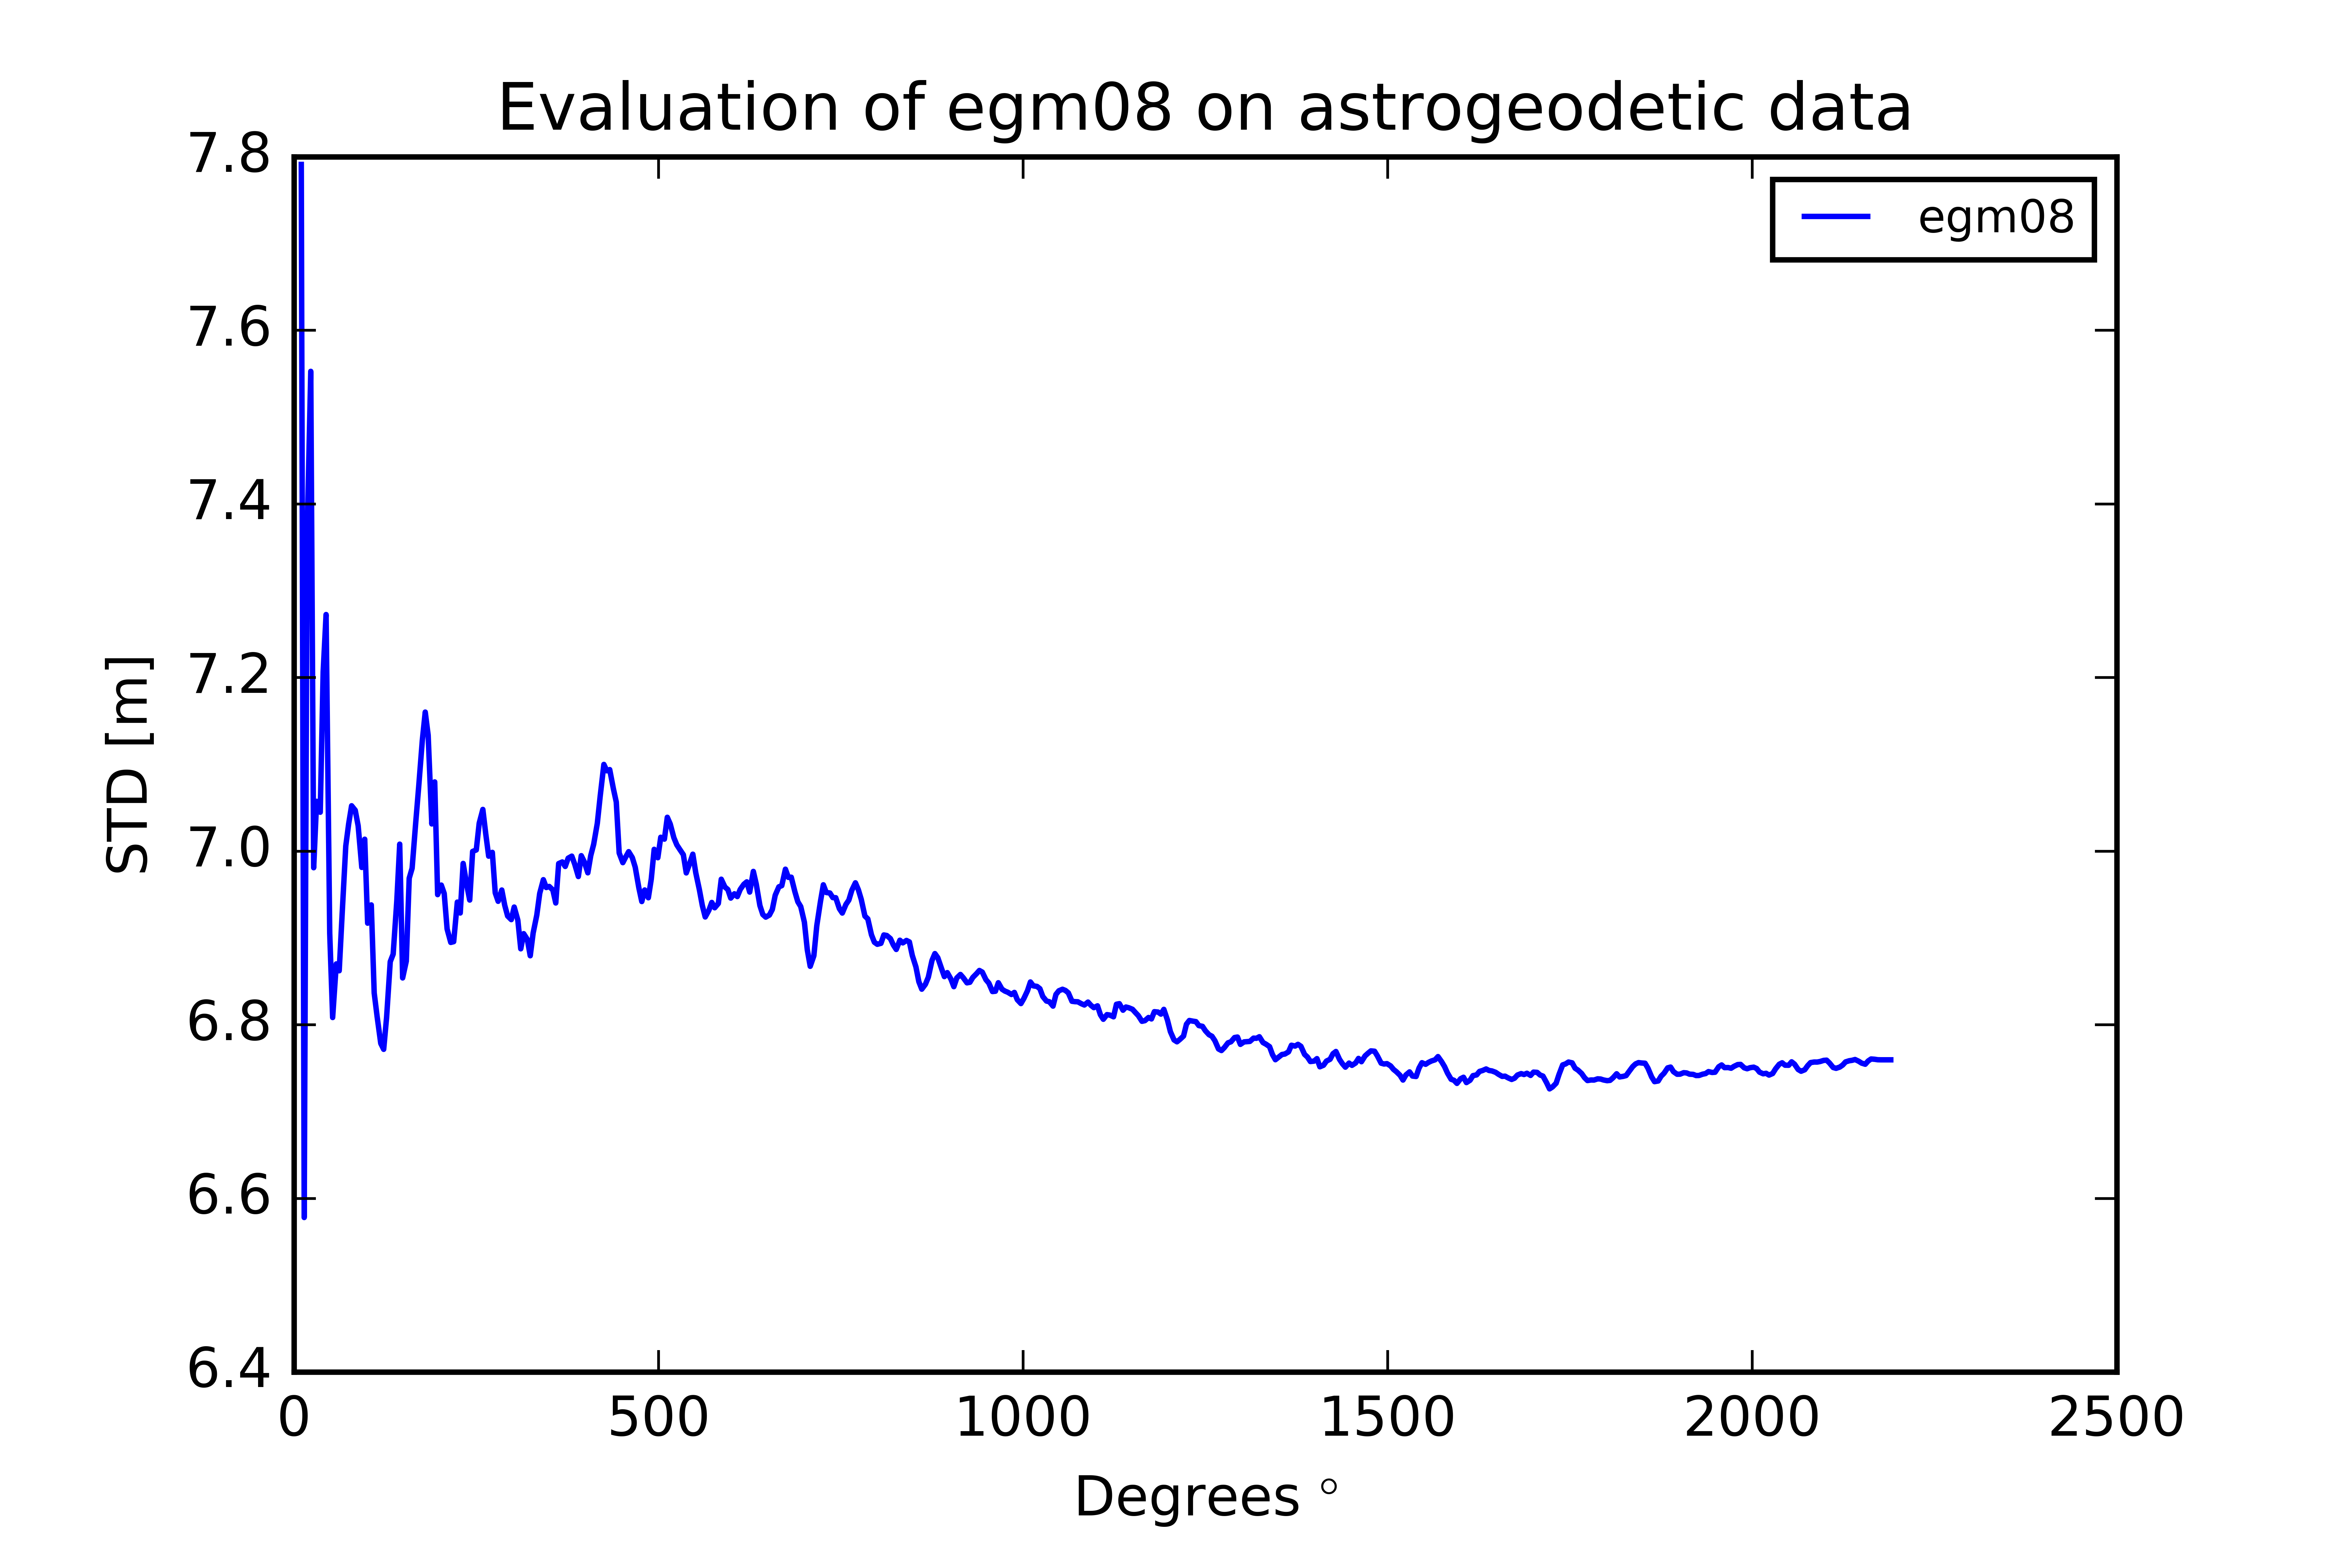
\includegraphics{Figures/egm08_figure.png}
      	\centering
      \end{figure}
      
      
      \begin{figure}[t]
      	\caption{std behaviour with the change of degrees}
      	\label{itu_grace16_figure}
      	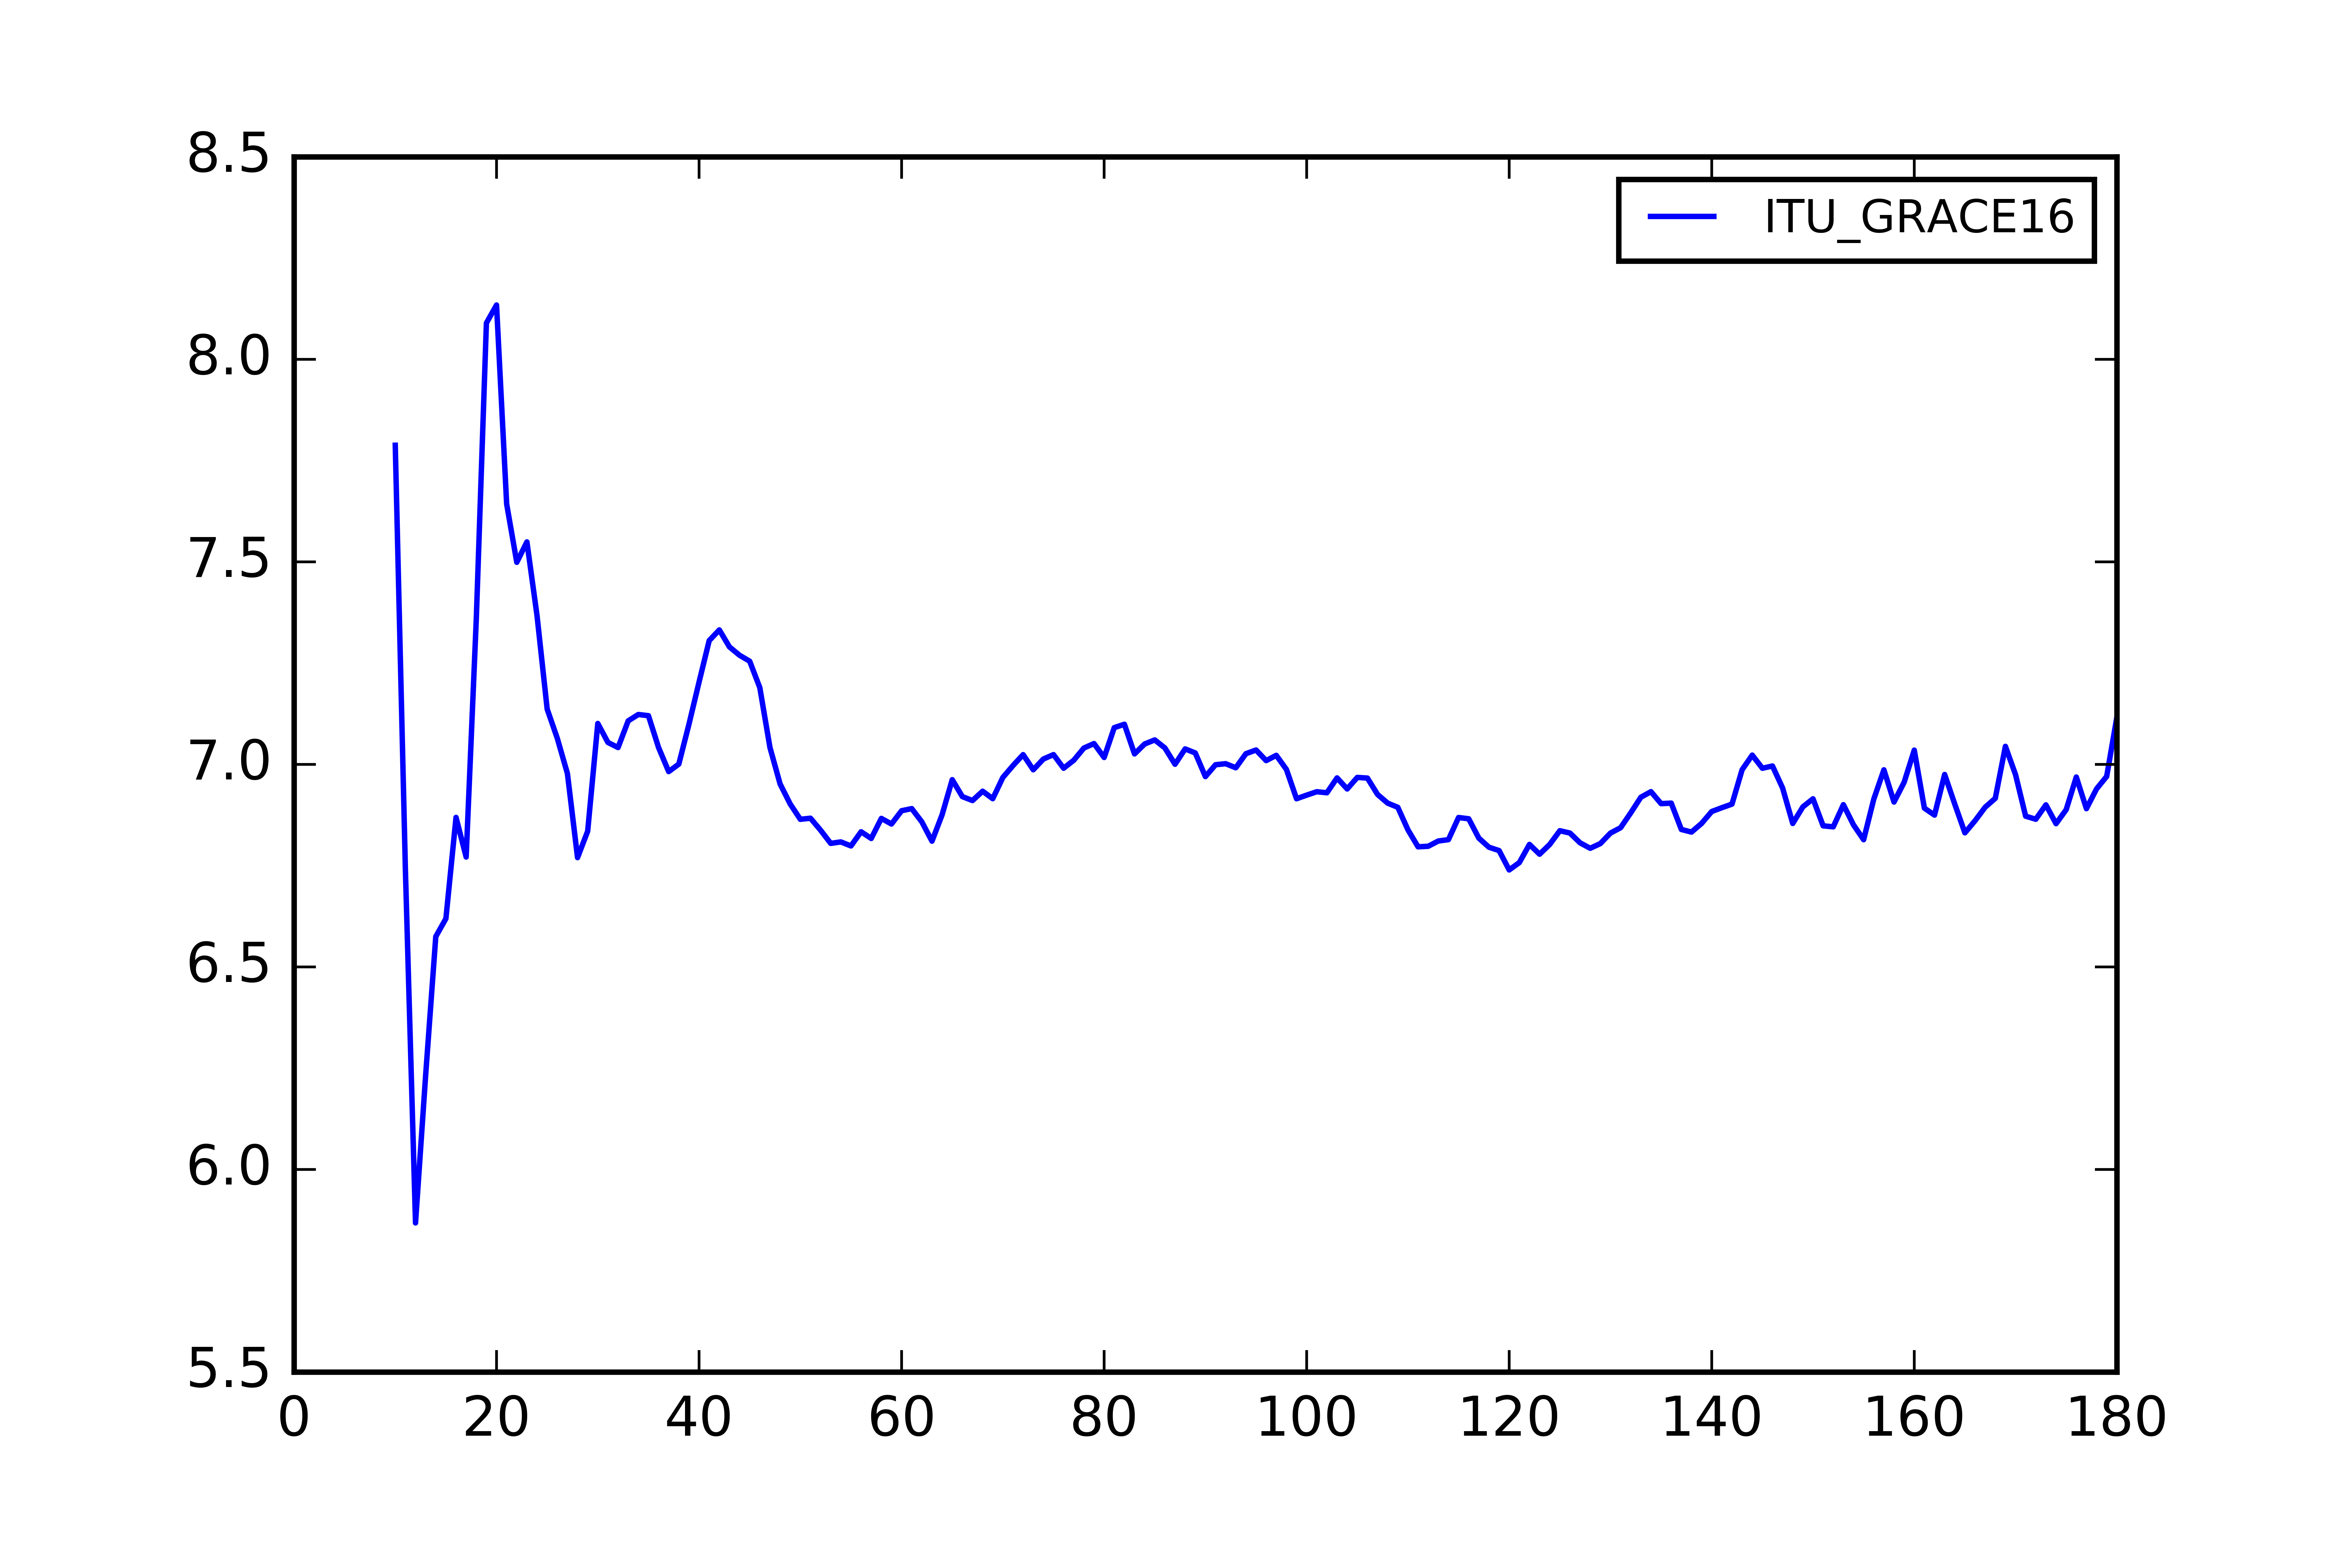
\includegraphics{Figures/ITU_GRACE16_figure.png}
      	\centering
      \end{figure}
      
      
      \begin{figure}[t]
      	\caption{std behaviour with the change of degrees}
      	\label{itu_ggc16_figure}
      	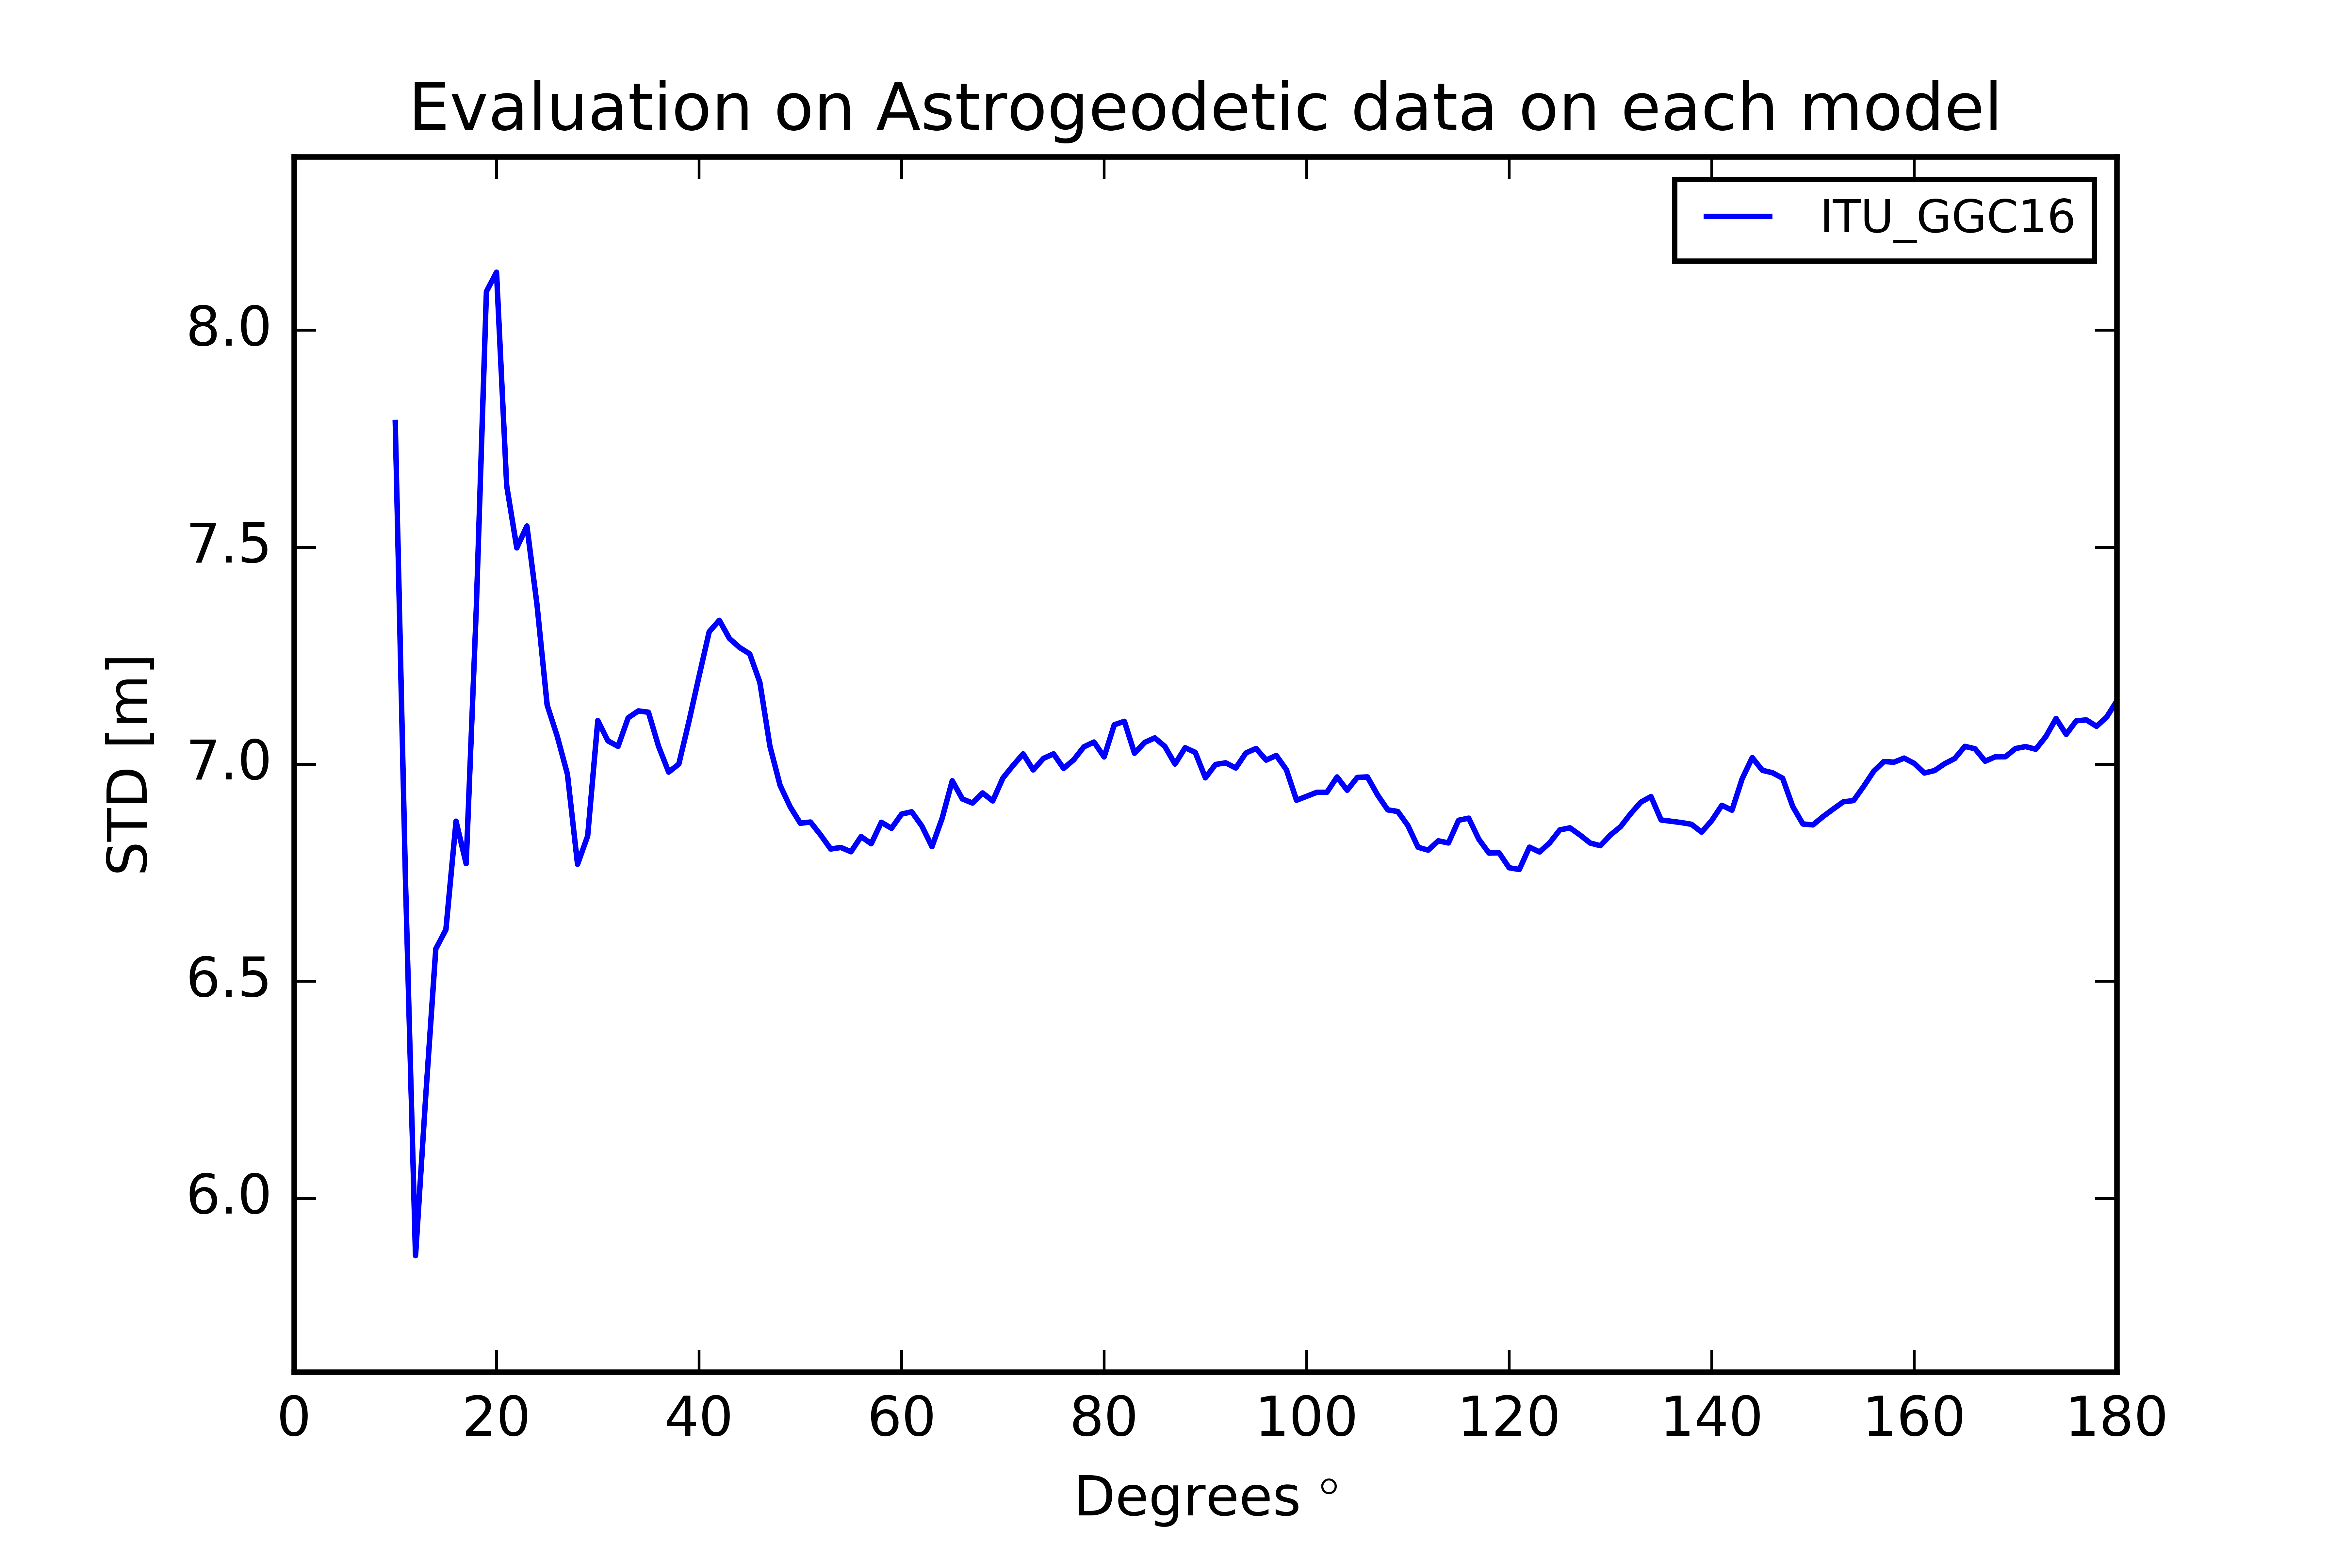
\includegraphics{Figures/ITU_GGC16_figure.png}
      	\centering
      \end{figure}
      
      
      \begin{figure}[t]
      	\caption{std behaviour with the change of degrees}
      	\label{geco_figure}
      	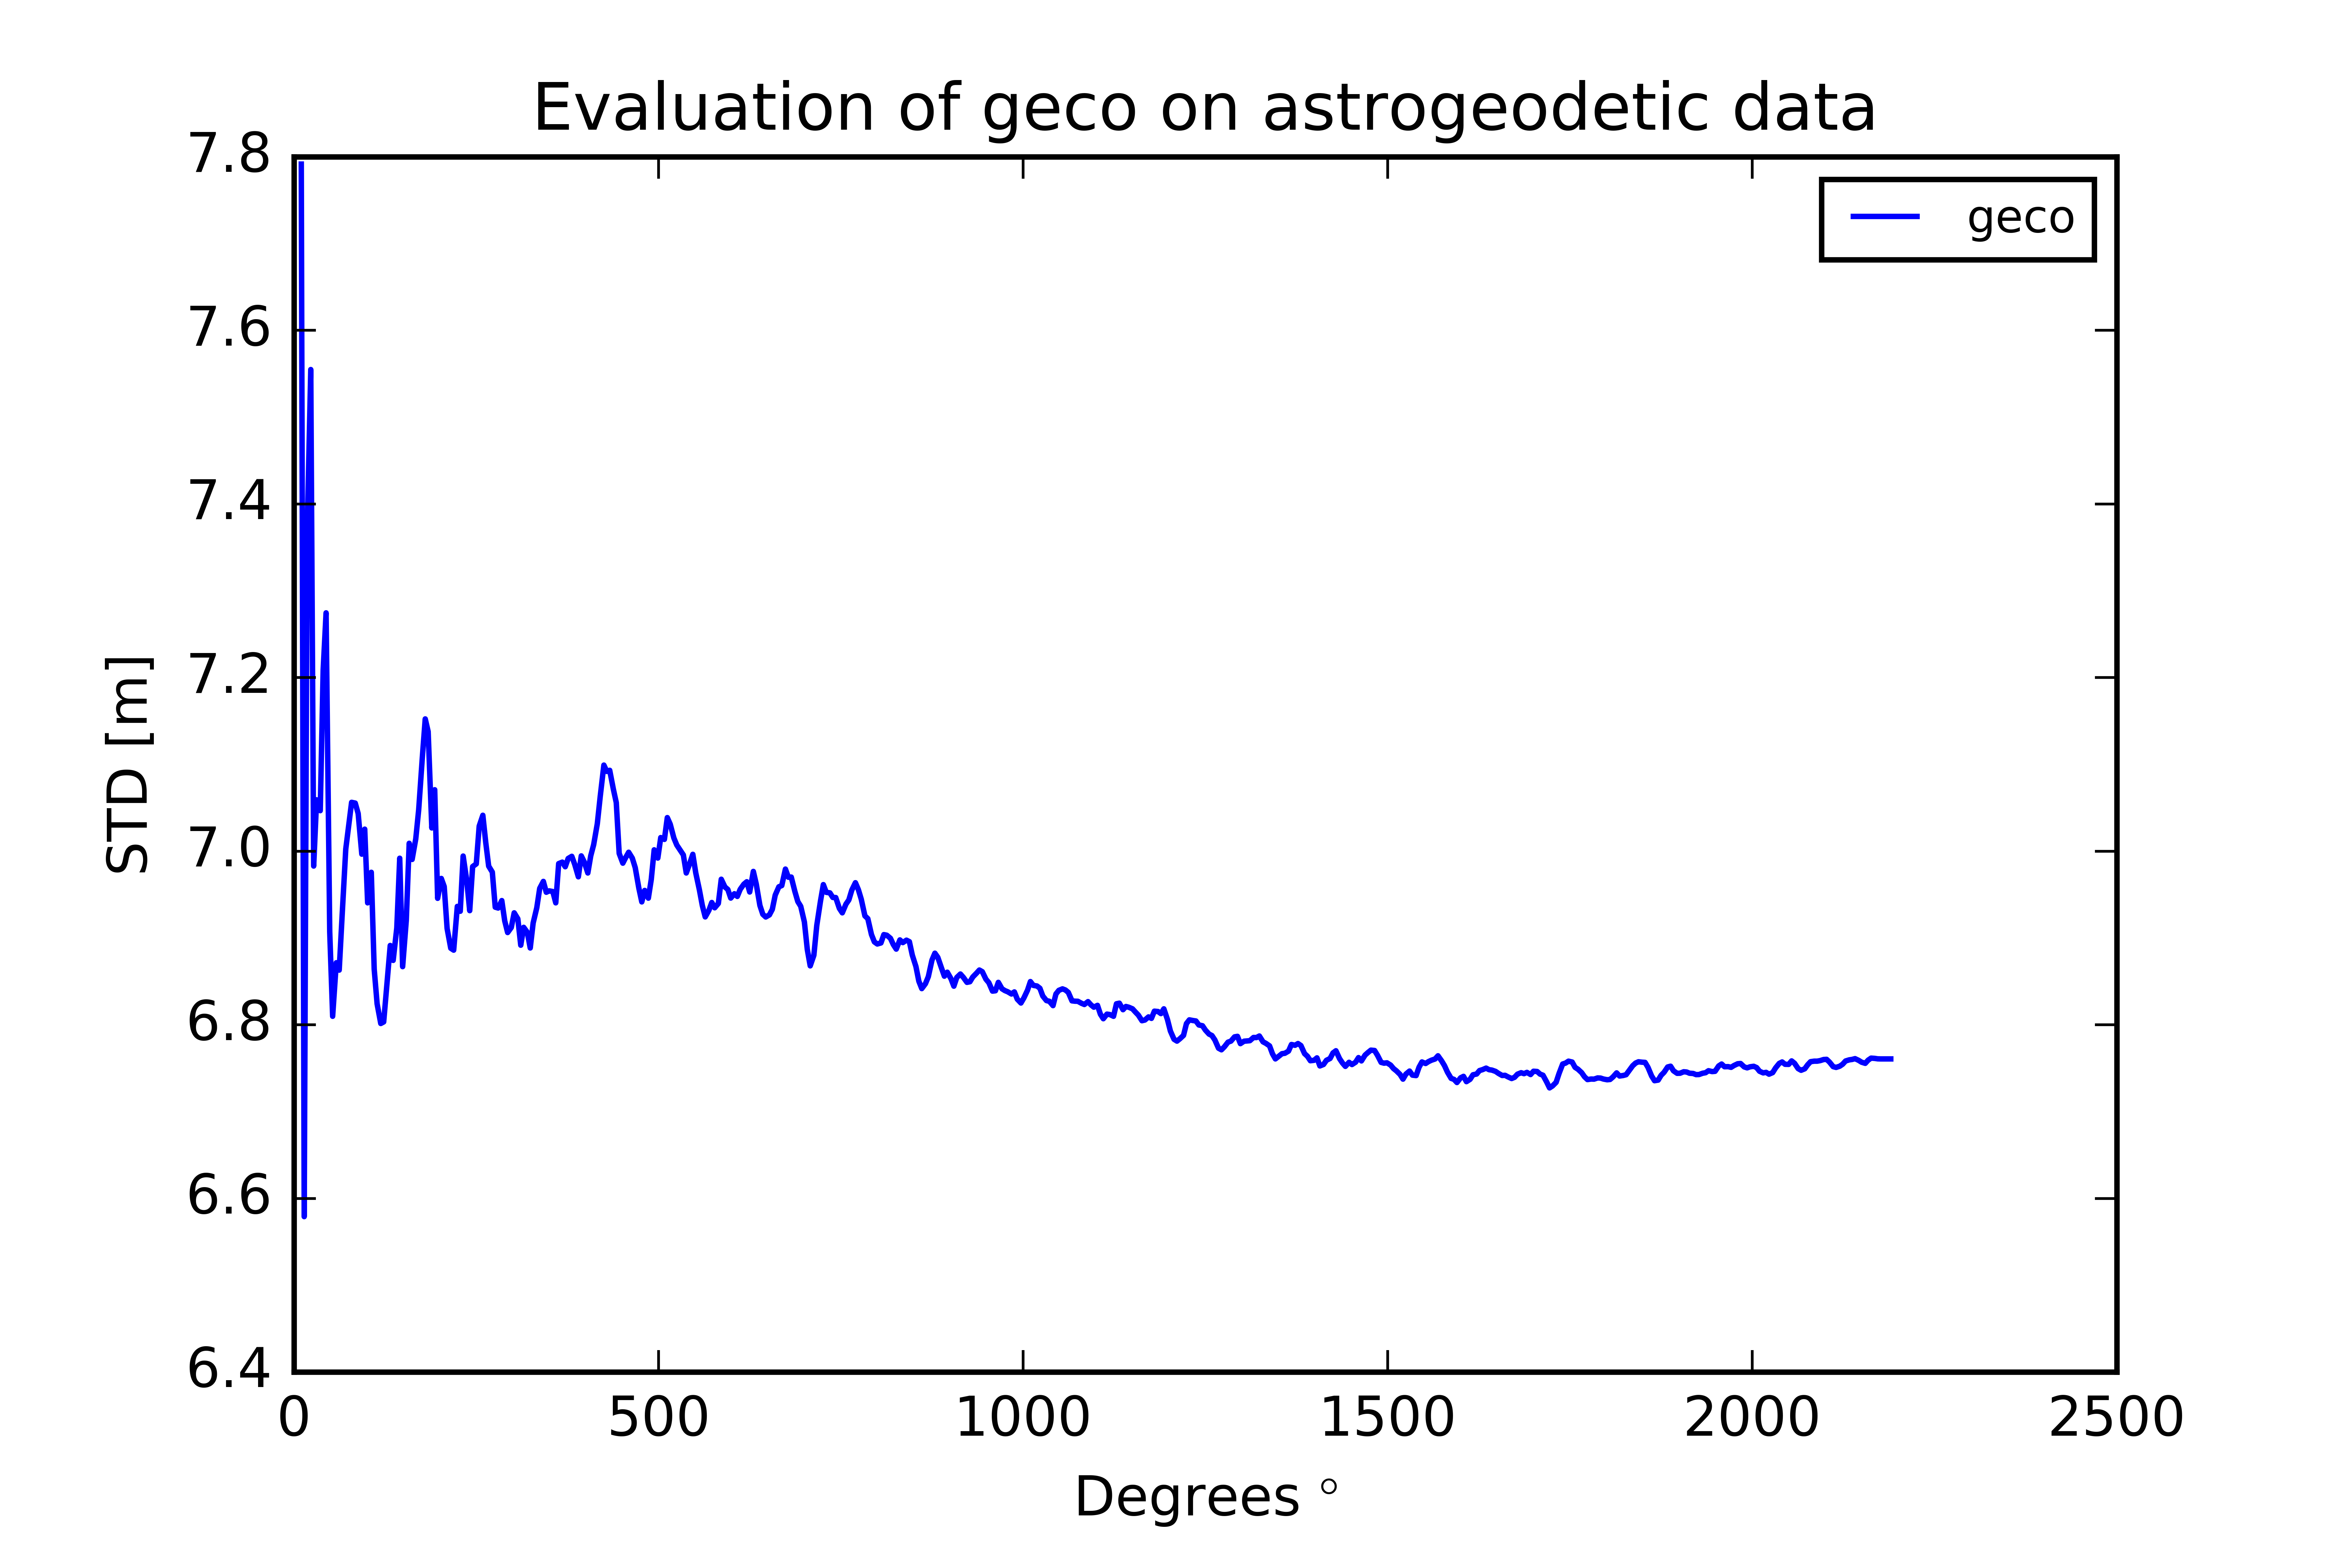
\includegraphics{Figures/geco_figure.png}
      	\centering
      \end{figure}
      
      \begin{figure}[t]
      	\caption{std behaviour with the change of degrees}
      	\label{eigen_6c4_figure}
      	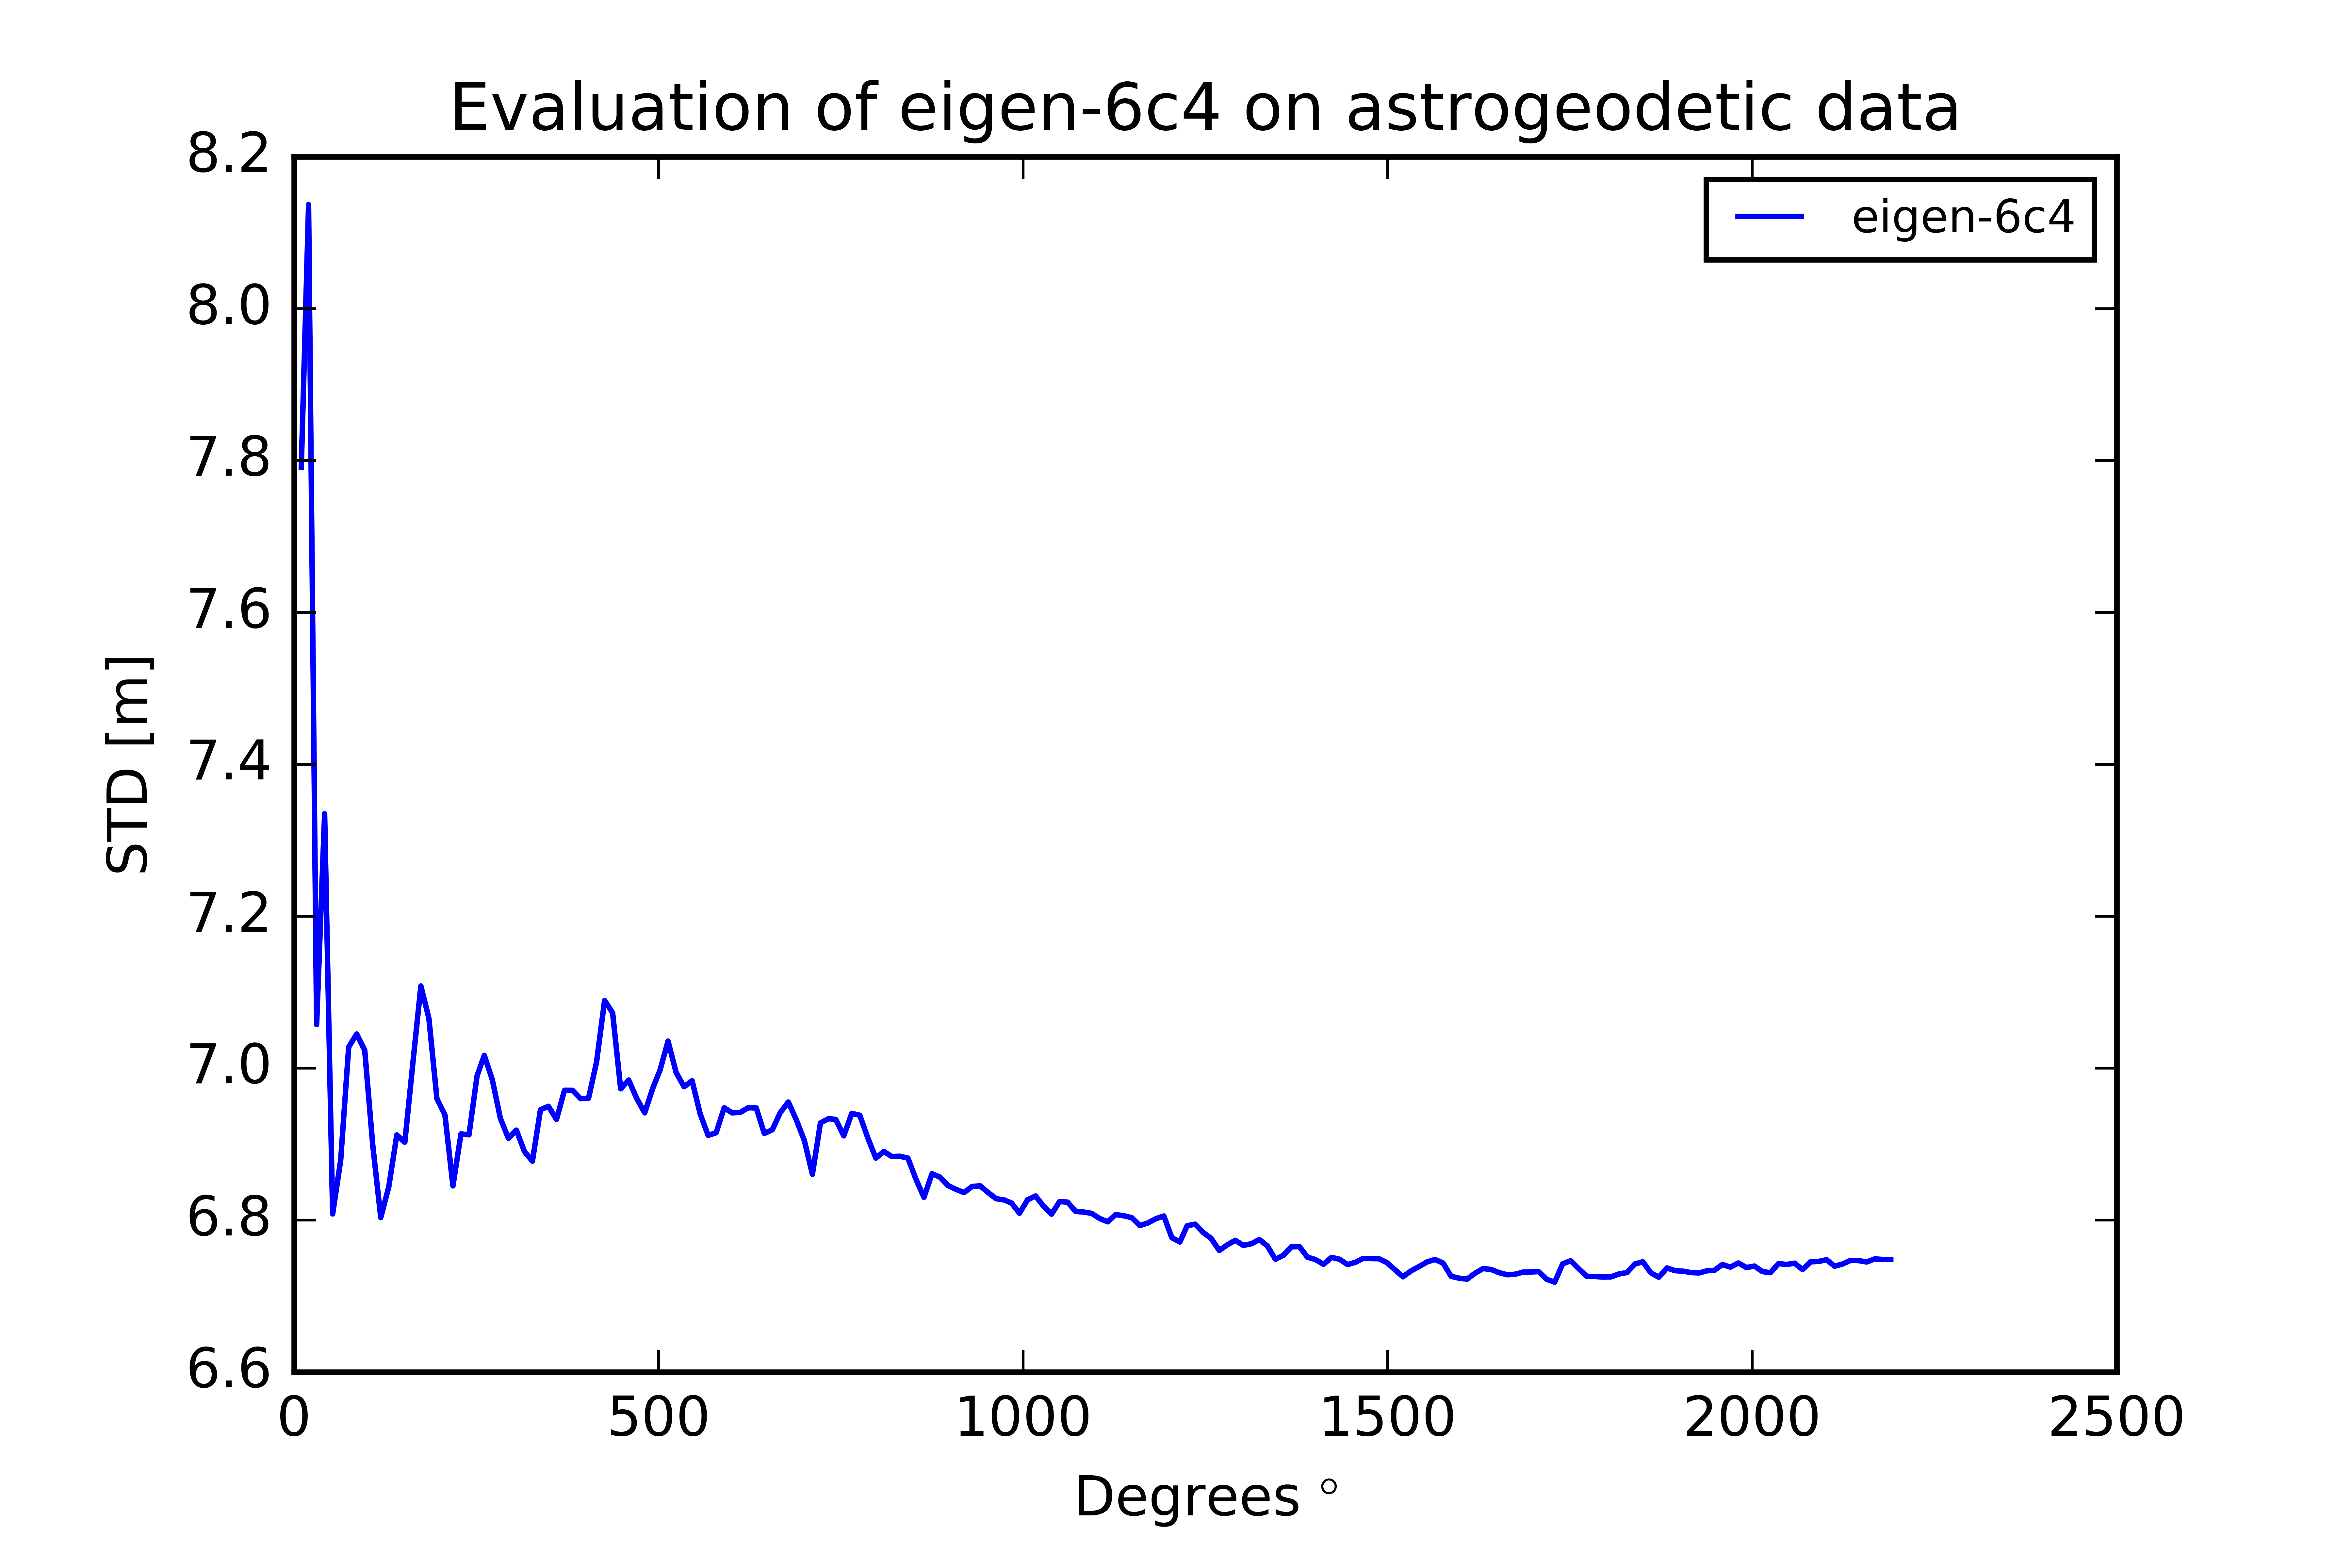
\includegraphics{Figures/eigen-6c4_figure.png}
      	\centering
      \end{figure}
      
      
        \begin{figure}[t]
           	\caption{Behavior of the five models truncated to the lowest model}
           	\label{eigen_6c4_figure}
           	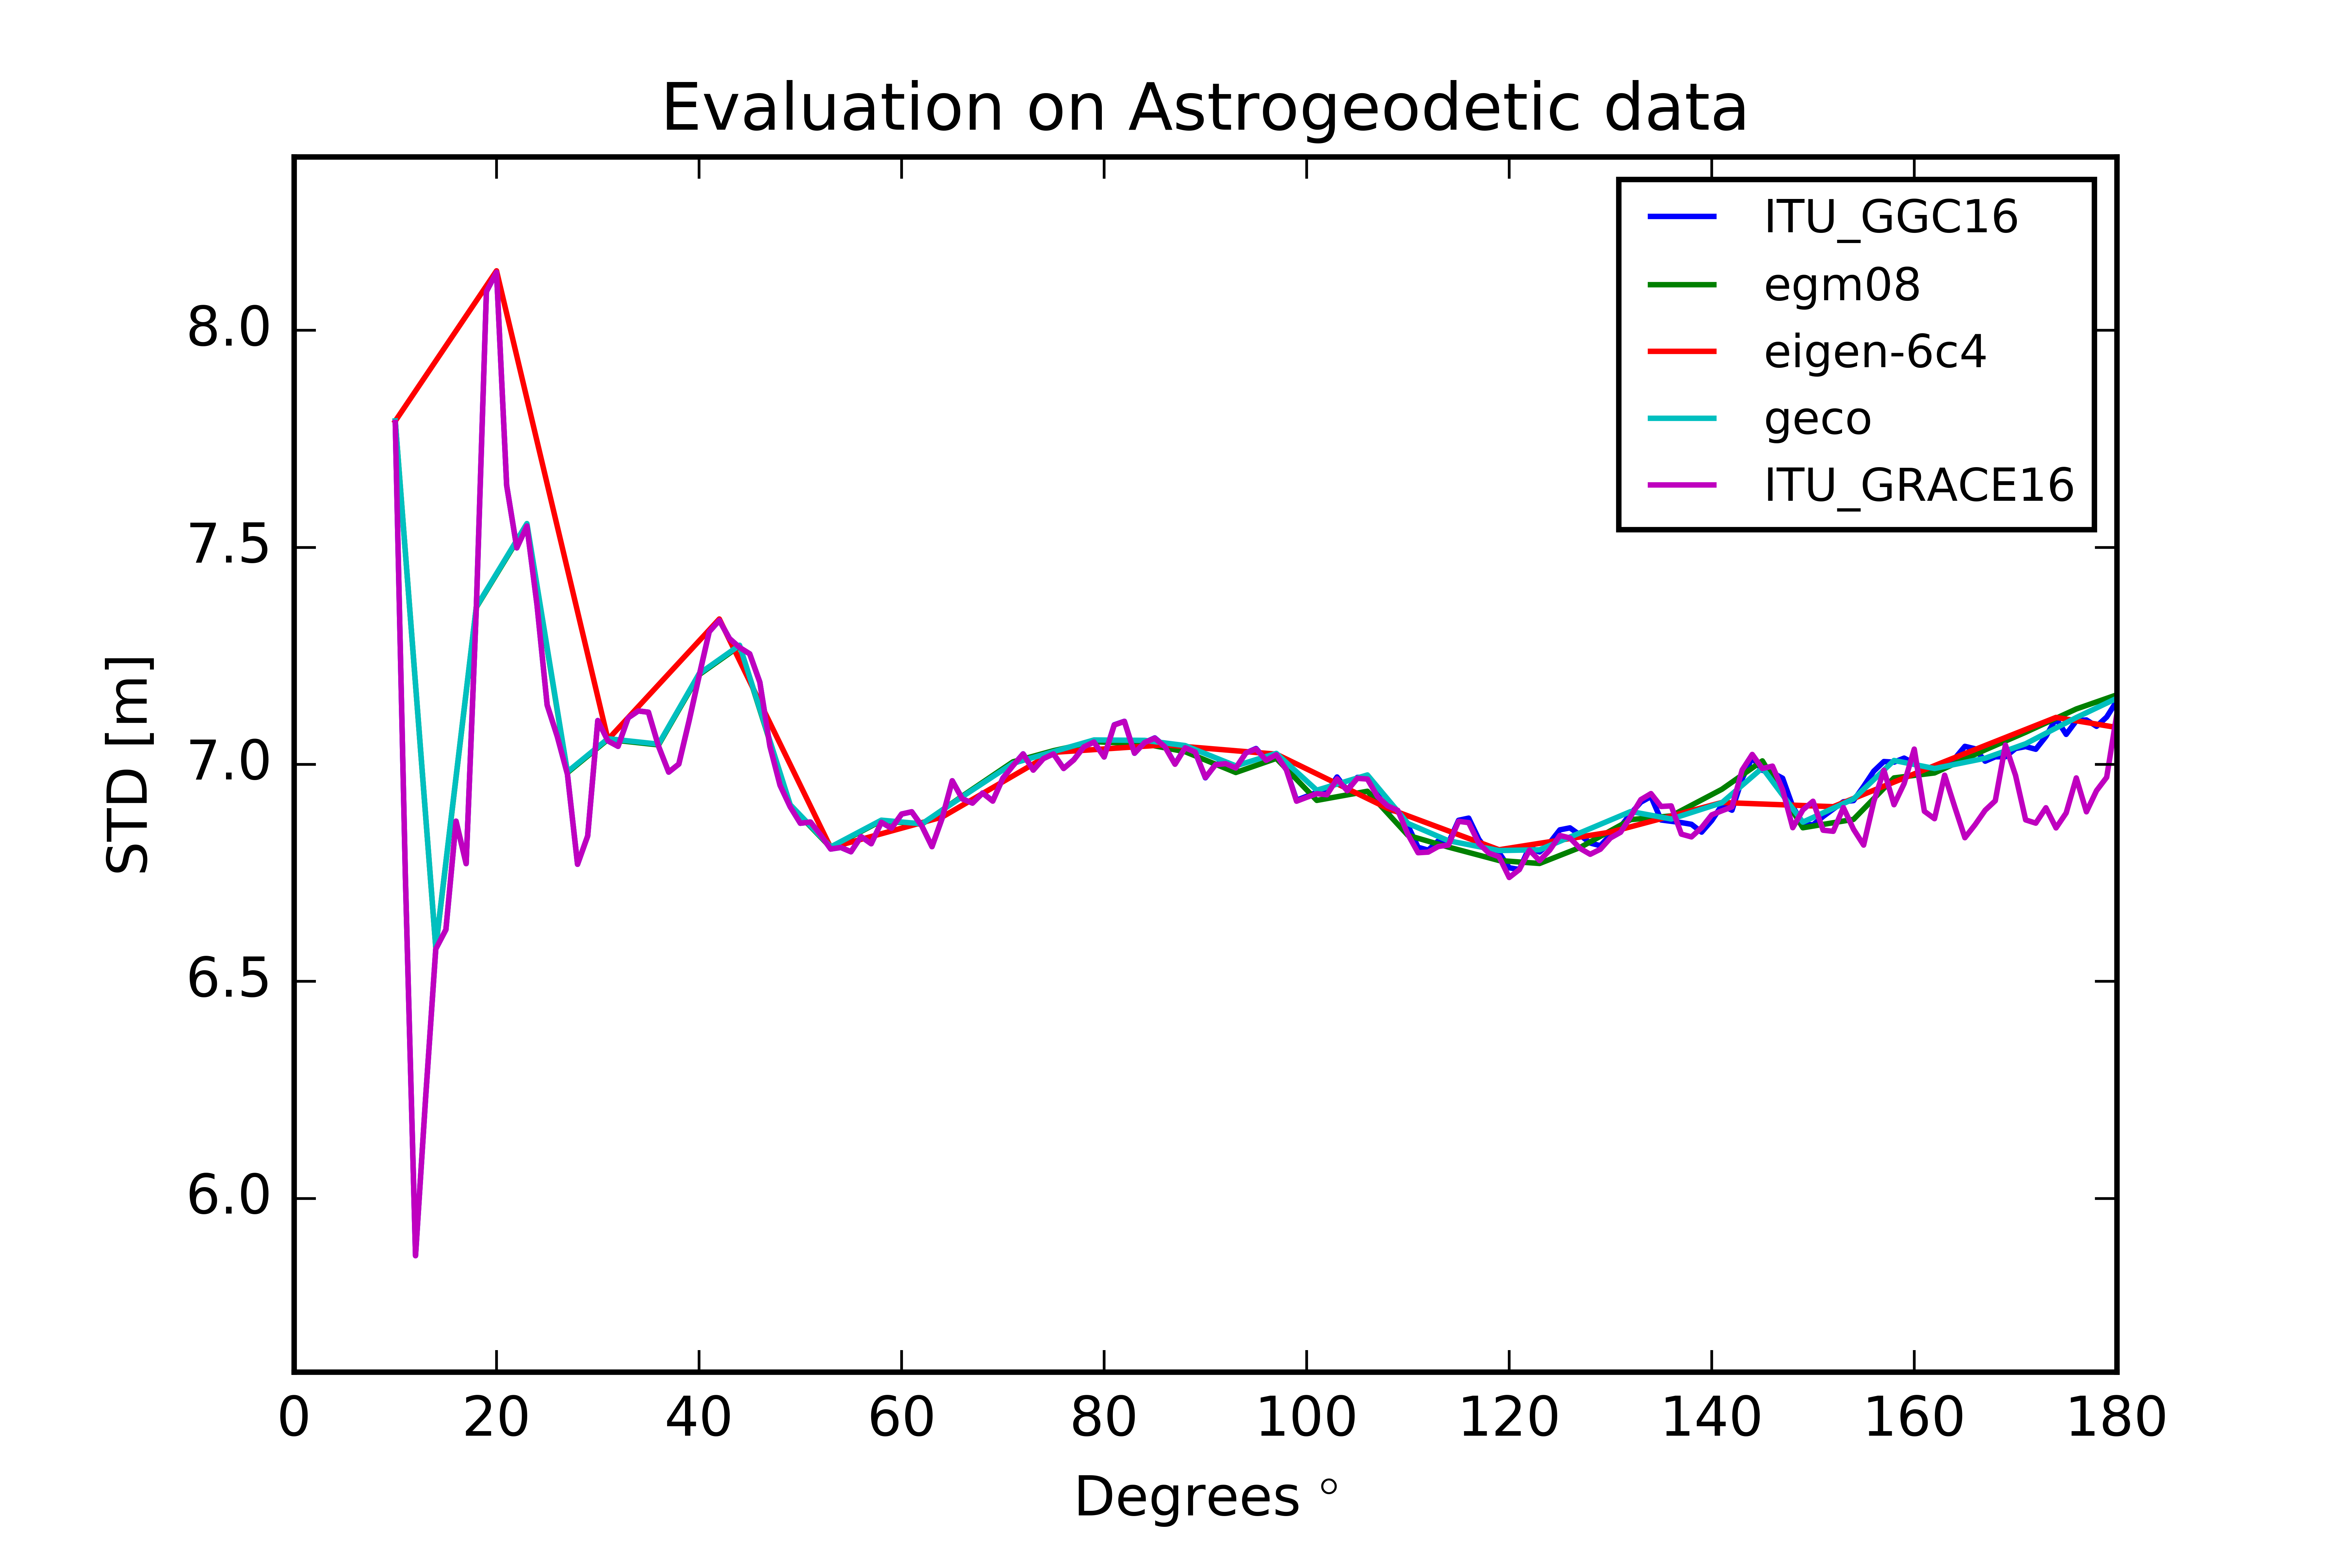
\includegraphics{Figures/grayscale_style.png}
           	\centering
        \end{figure}
        
        \section{Evaluation of GPS/Leveling data}
        The second dataset that we used is GPS/Leveling data. It consists of 24 GPS/leveling data that were collected from 2005-2008 from different geodetic networks ranging from $1^{st}$ order networks to $3^{rd}$ order networks. Our evaluation on GPS/leveling data shows that the std error has dropped from 5.86m to 0.365349m. ITU\_GRACE16 had a very strange trend in degrees > 150. The reason for that is due to the emission error that takes place in the higher degree of the satellite model.
        Another observation is that in all of our models, the best 5 models are dominant by the higher degrees, 150 for ITU\_GCC16 and (669, 665, and 674) for EGM2008. For EIGEN-6C4 there is 667, 327, and 678. GECO had a near result to that recorded by ITU\_GCC16 (the difference is 0.000131m), has three high degree models in its 5 best models, 669, 674, and 263. The definition of high order models is quite arbitrary, but use the score that degrees > 100 is called high degree models, else are low degree models. In our best 20 models (based on std) for all models, 18 of the 20 are classified as high degree models which is 90\% of the total 20 models. We conclude that using high order/degree models often leads to a better results. It's true for the global representation of the gravitational functionals that ``the \textit{higher} is the \textit{better}", but that does not always hold true for the local case. Hence, the evaluation of different degrees of the model on local data. We evaluated three high models together (EGM2008, EIGEN-6C-4, and GECO), the results on the lower degrees (< 900) seems to be a bit noisy (a few peaks occur), but for the higher degrees the results were very stable. GECO and EIGEN-6C4 has always surpassed those of EGM2008, even though some of their degrees are derived from EGM2008. There a constant difference between EGM2008 and GECO and EIGEN-6C4 results, they all have the same trend. The magnitude of the difference between GECO and EIGEN-6C4 is constant, which lead us to believe that there were a systematic error(s) in EGM2008 and they were resolved in the latter models. 
          \begin{table}[]
          	\centering
          	\caption{Top 5 degrees for model ITU\_GRACE on GPS/leveling data}
          	\label{table:ggm_models}
          	\begin{tabular}{@{}lll@{}}
          		\toprule
          		\emph{degree} & std $\sigma$ [m]  & difference\\ \midrule
          		46 &0.367751&    0.571191\\
          		152 &0.369840&   0.417293\\
          		149 &0.373809 &  0.127576\\
          		29 &0.3739635 &  -0.027817\\
          		30 &0.374076  & -1.040373\\
          		\bottomrule
          		
          	\end{tabular}
          \end{table}
          
            \begin{table}[]
            	\centering
            	\caption{Top 5 degrees for model ITU\_GGC on GPS/leveling data}
            	\label{table:ggm_models}
            	\begin{tabular}{@{}lll@{}}
            		\toprule
            		\emph{degree} & std $\sigma$ [m]  & difference\\ \midrule
            		149 &0.365349&    0.330661\\
            		150 &0.366355&   0.354195\\
            		46 &0.367751 &  0.571312\\
            		148 &0.368081 &  0.300463\\
            		152 &0.368113  & 0.509021\\
            		\bottomrule
            		
            	\end{tabular}
            \end{table}
            
            
              \begin{table}[]
              	\centering
              	\caption{Top 5 degrees for model EGM2008 on GPS/leveling data}
              	\label{table:ggm_models}
              	\begin{tabular}{@{}lll@{}}
              		\toprule
              		\emph{degree} & std $\sigma$ [m]  & difference\\ \midrule
              		669 &0.373804&    0.487649\\
              		665 &0.373929&   0.486516\\
              		149 &0.375045 &  0.407975\\
              		674 &0.376249 &  0.486830\\
              		31 &0.376251  & 1.316226\\
              		\bottomrule
              		
              	\end{tabular}
              \end{table}
              
              \begin{table}
               	\centering
               	\caption{Top 5 degrees for model EIGEN-6C4 on GPS/leveling data}
               	\label{table:ggm_models}
               	\begin{tabular}{@{}lll@{}}
               		\toprule
               		\emph{degree} & std $\sigma$ [m]  & difference\\ \midrule
               		667 &0.368126&    0.371325\\
               		152 &0.368243&   0.460720\\
               		327 &0.3713845 &  0.400191\\
               		678 &0.372534 &  0.372325\\
               		261 &0.372603  & 0.352102\\
               		\bottomrule
               		
               	\end{tabular}
               \end{table}
        
          \begin{table}[]
          	\centering
          	\caption{Top 5 degrees for model GECO on GPS/leveling data}
          	\label{table:ggm_models}
          	\begin{tabular}{@{}lll@{}}
          		\toprule
          		\emph{degree} & std $\sigma$ [m]  & difference\\ \midrule
          		149 &0.365480&    0.304553\\
          		669 &0.369906&   0.379220\\
          		665 &0.370001 &  0.378087\\
          		263 &0.370542 &  0.367333\\
          		674 &0.372194  & 0.378396\\
          		\bottomrule
          		
          	\end{tabular}
          \end{table}
        
        
        \begin{figure}[t]
        	\caption{Evaluation of our GGM on GPS/leveling data}
        	\label{sudan_data}
        	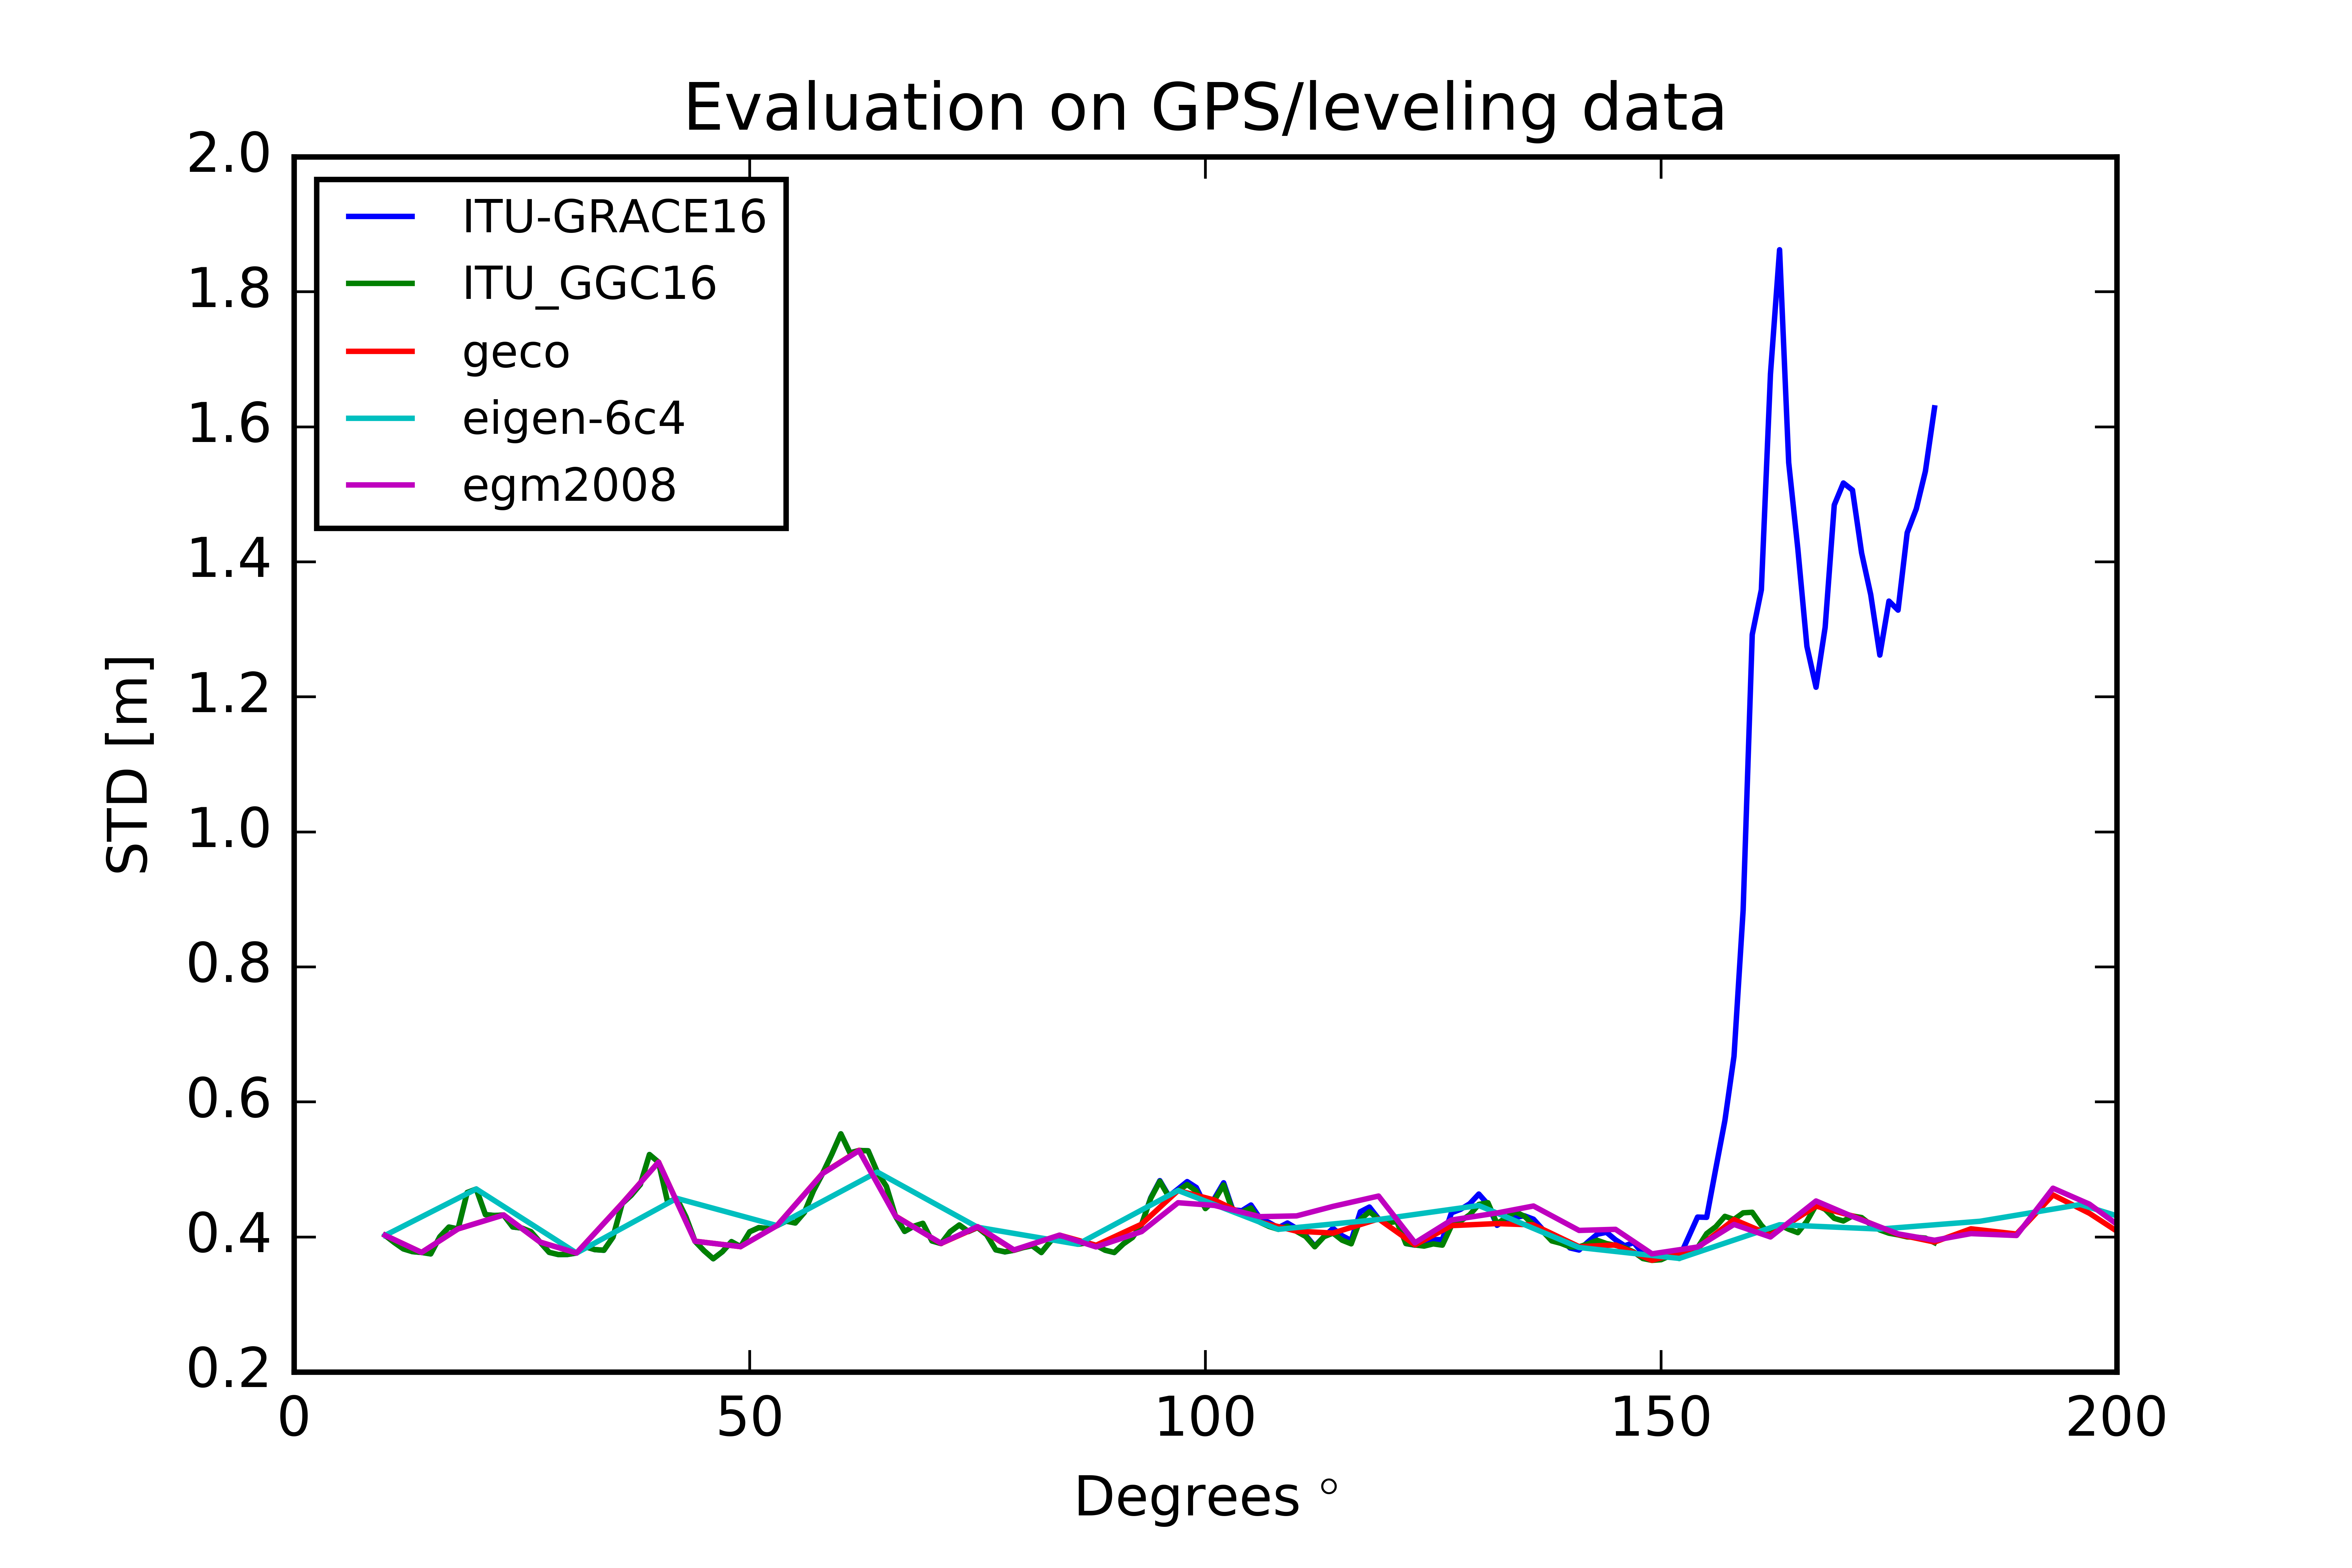
\includegraphics{Figures/classic_style.png}
        	\centering
        \end{figure}
        
        
        \begin{figure}[t]
        	\caption{Evaluation of EGM2008 on GPS/leveling data}
        	\label{sudan_data}
        	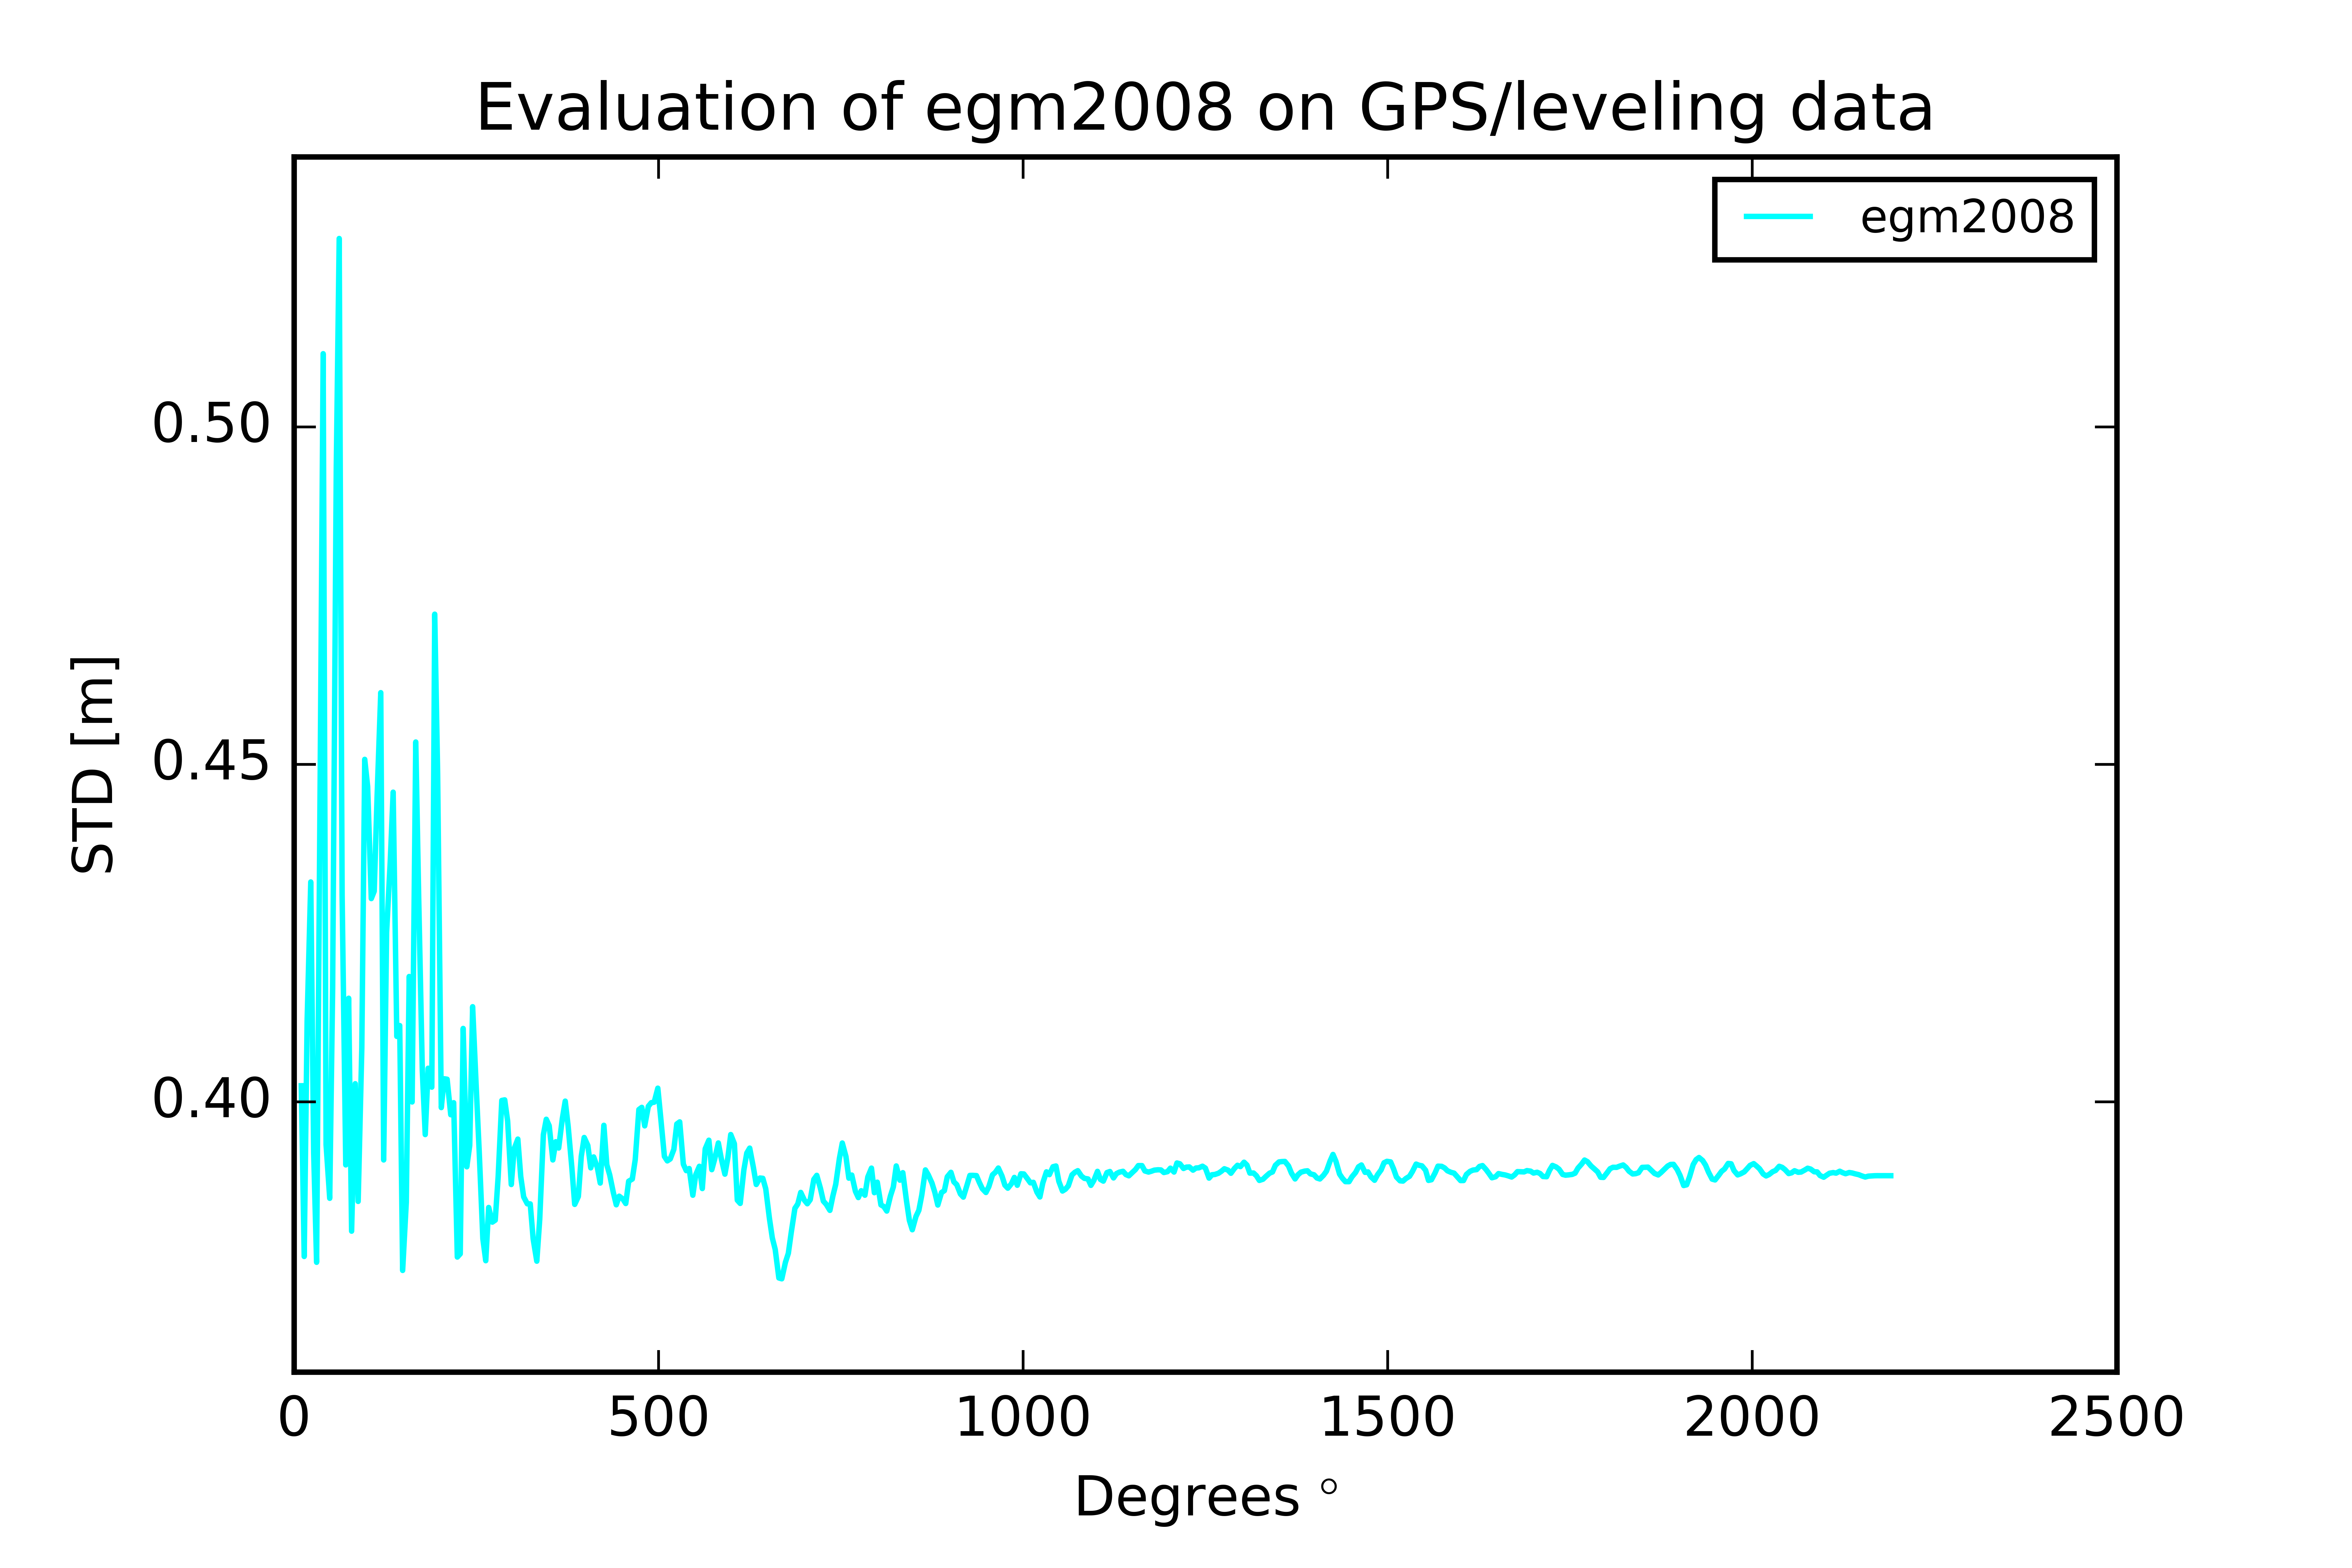
\includegraphics{Figures/egm2008_gps_figure.png}
        	\centering
        \end{figure}
        
        
        \begin{figure}[t]
        	\caption{Evaluation of ITU\_GRACE16 on GPS/leveling data}
        	\label{sudan_data}
        	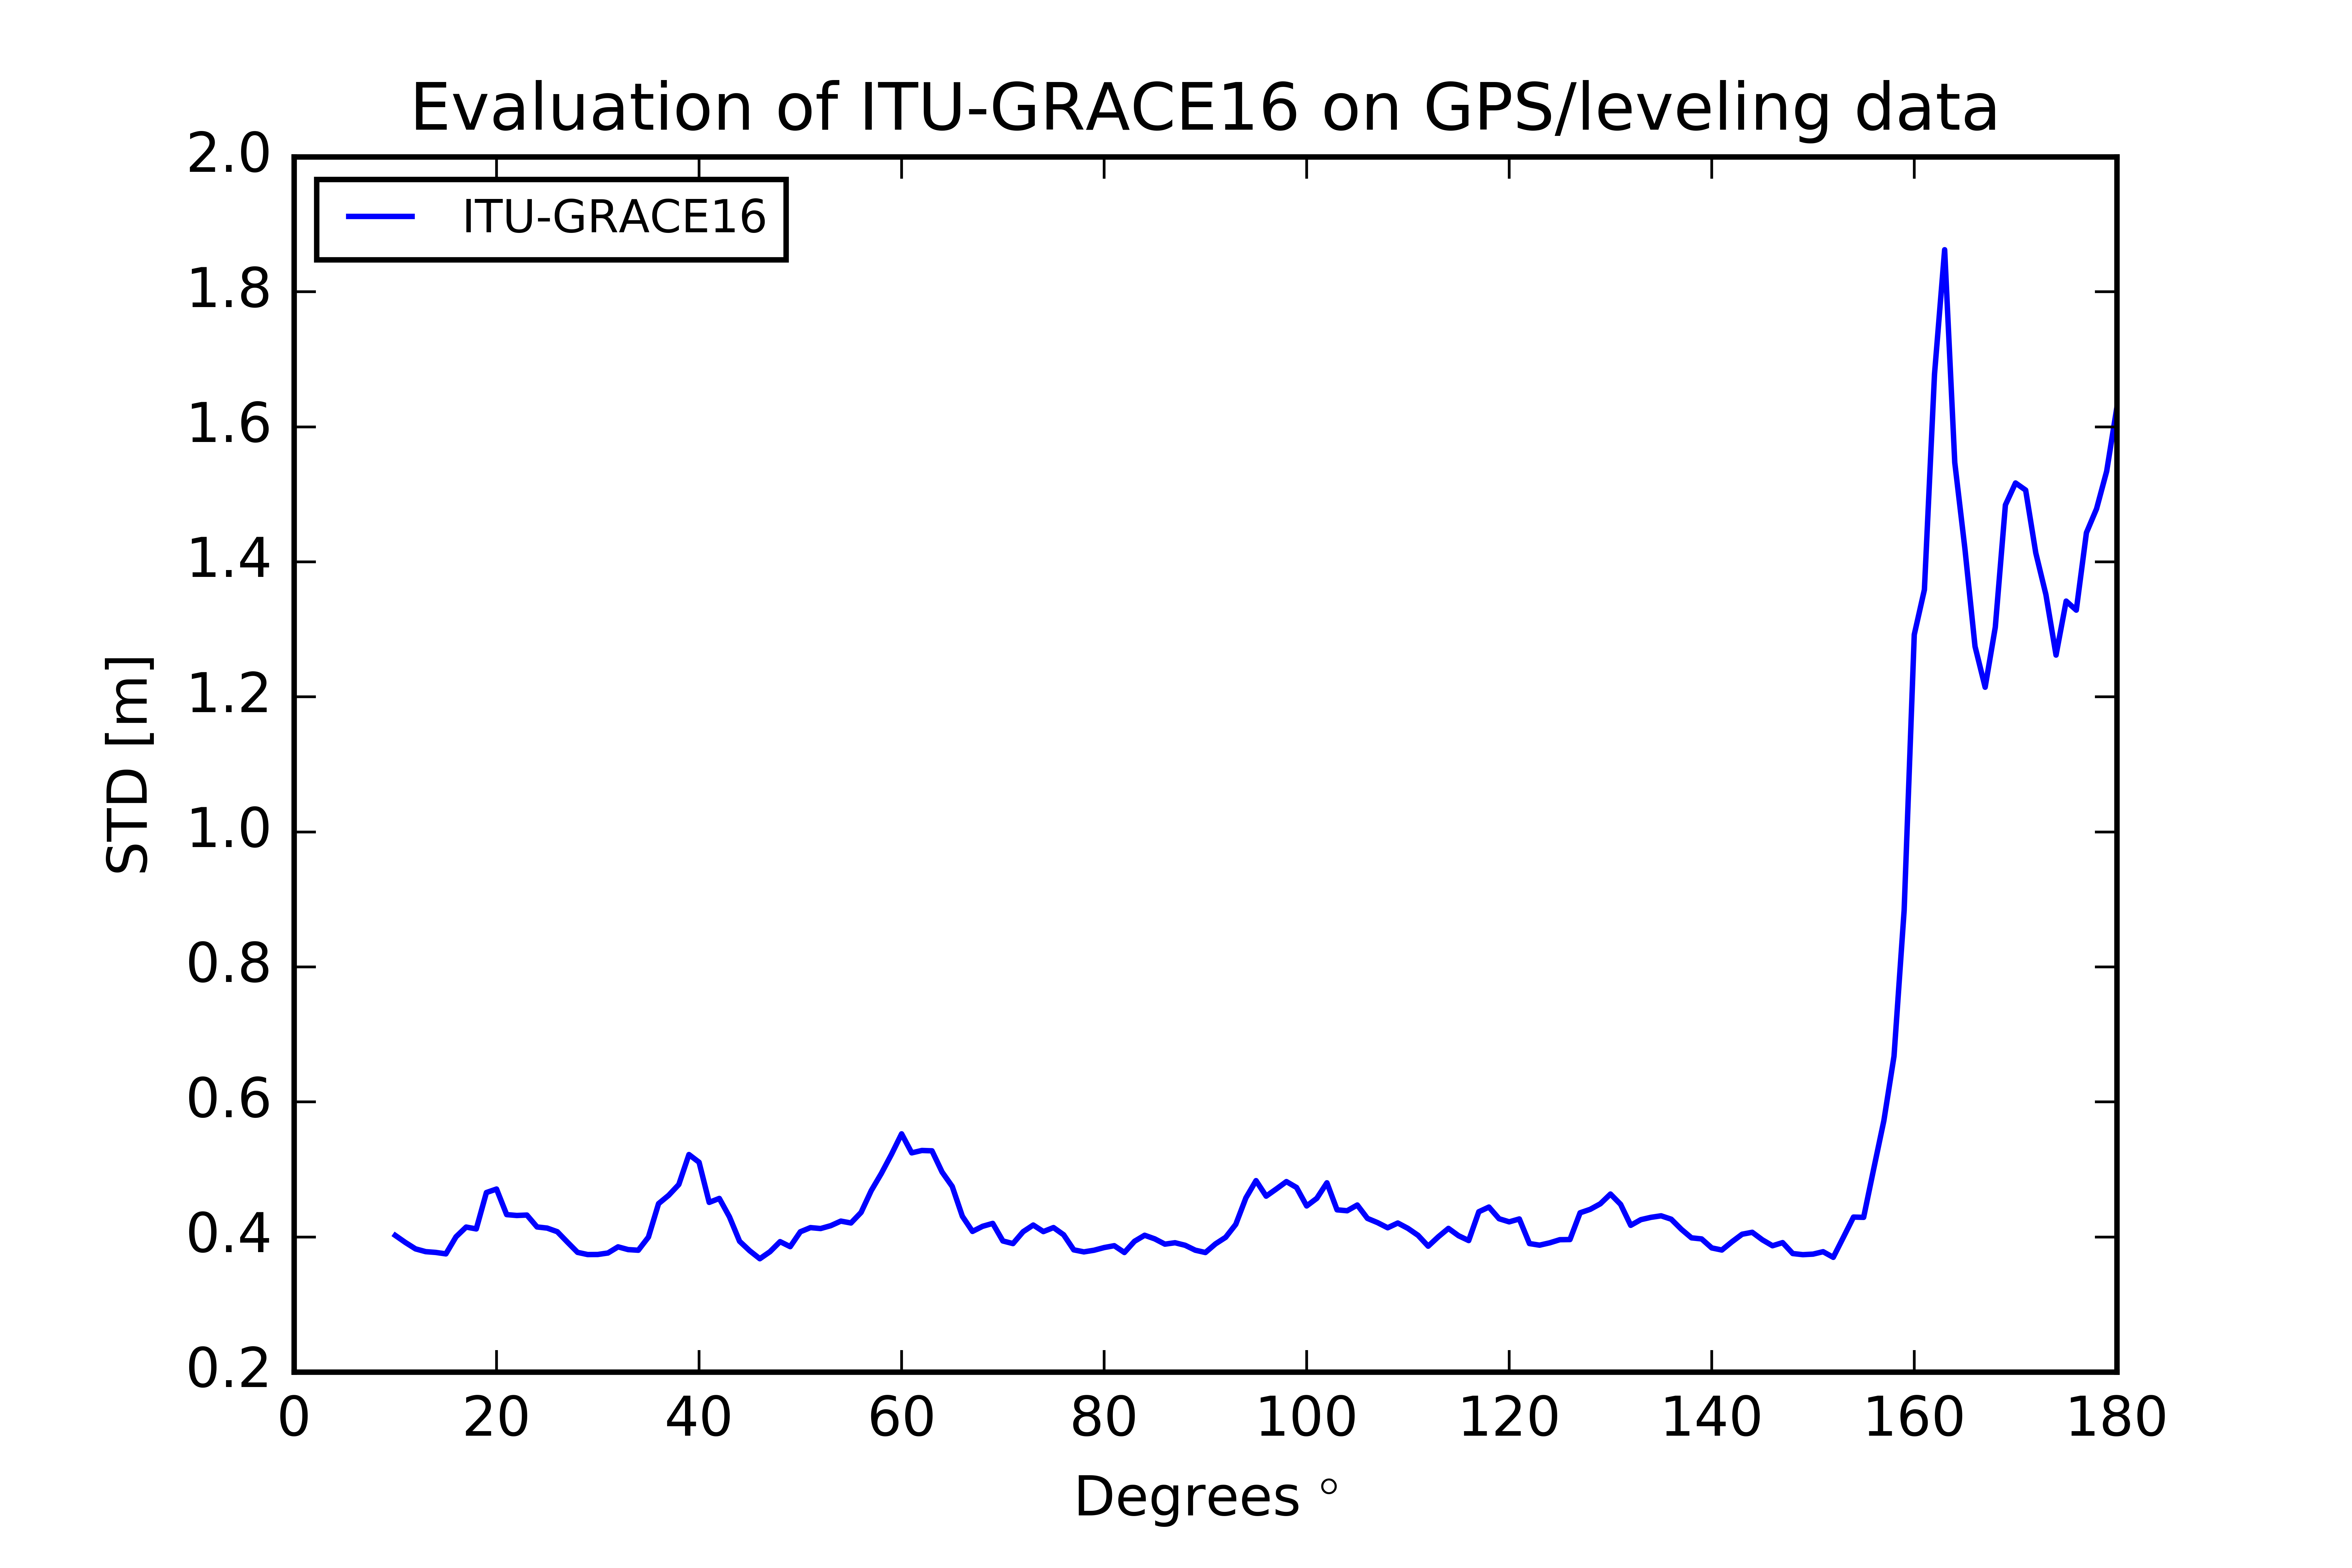
\includegraphics{Figures/ITU-GRACE16_gps_figure.png}
        	\centering
        \end{figure}
        
        
        \begin{figure}[t]
        	\caption{Evaluation of ITU\_GGC16 on GPS/leveling data}
        	\label{sudan_data}
        	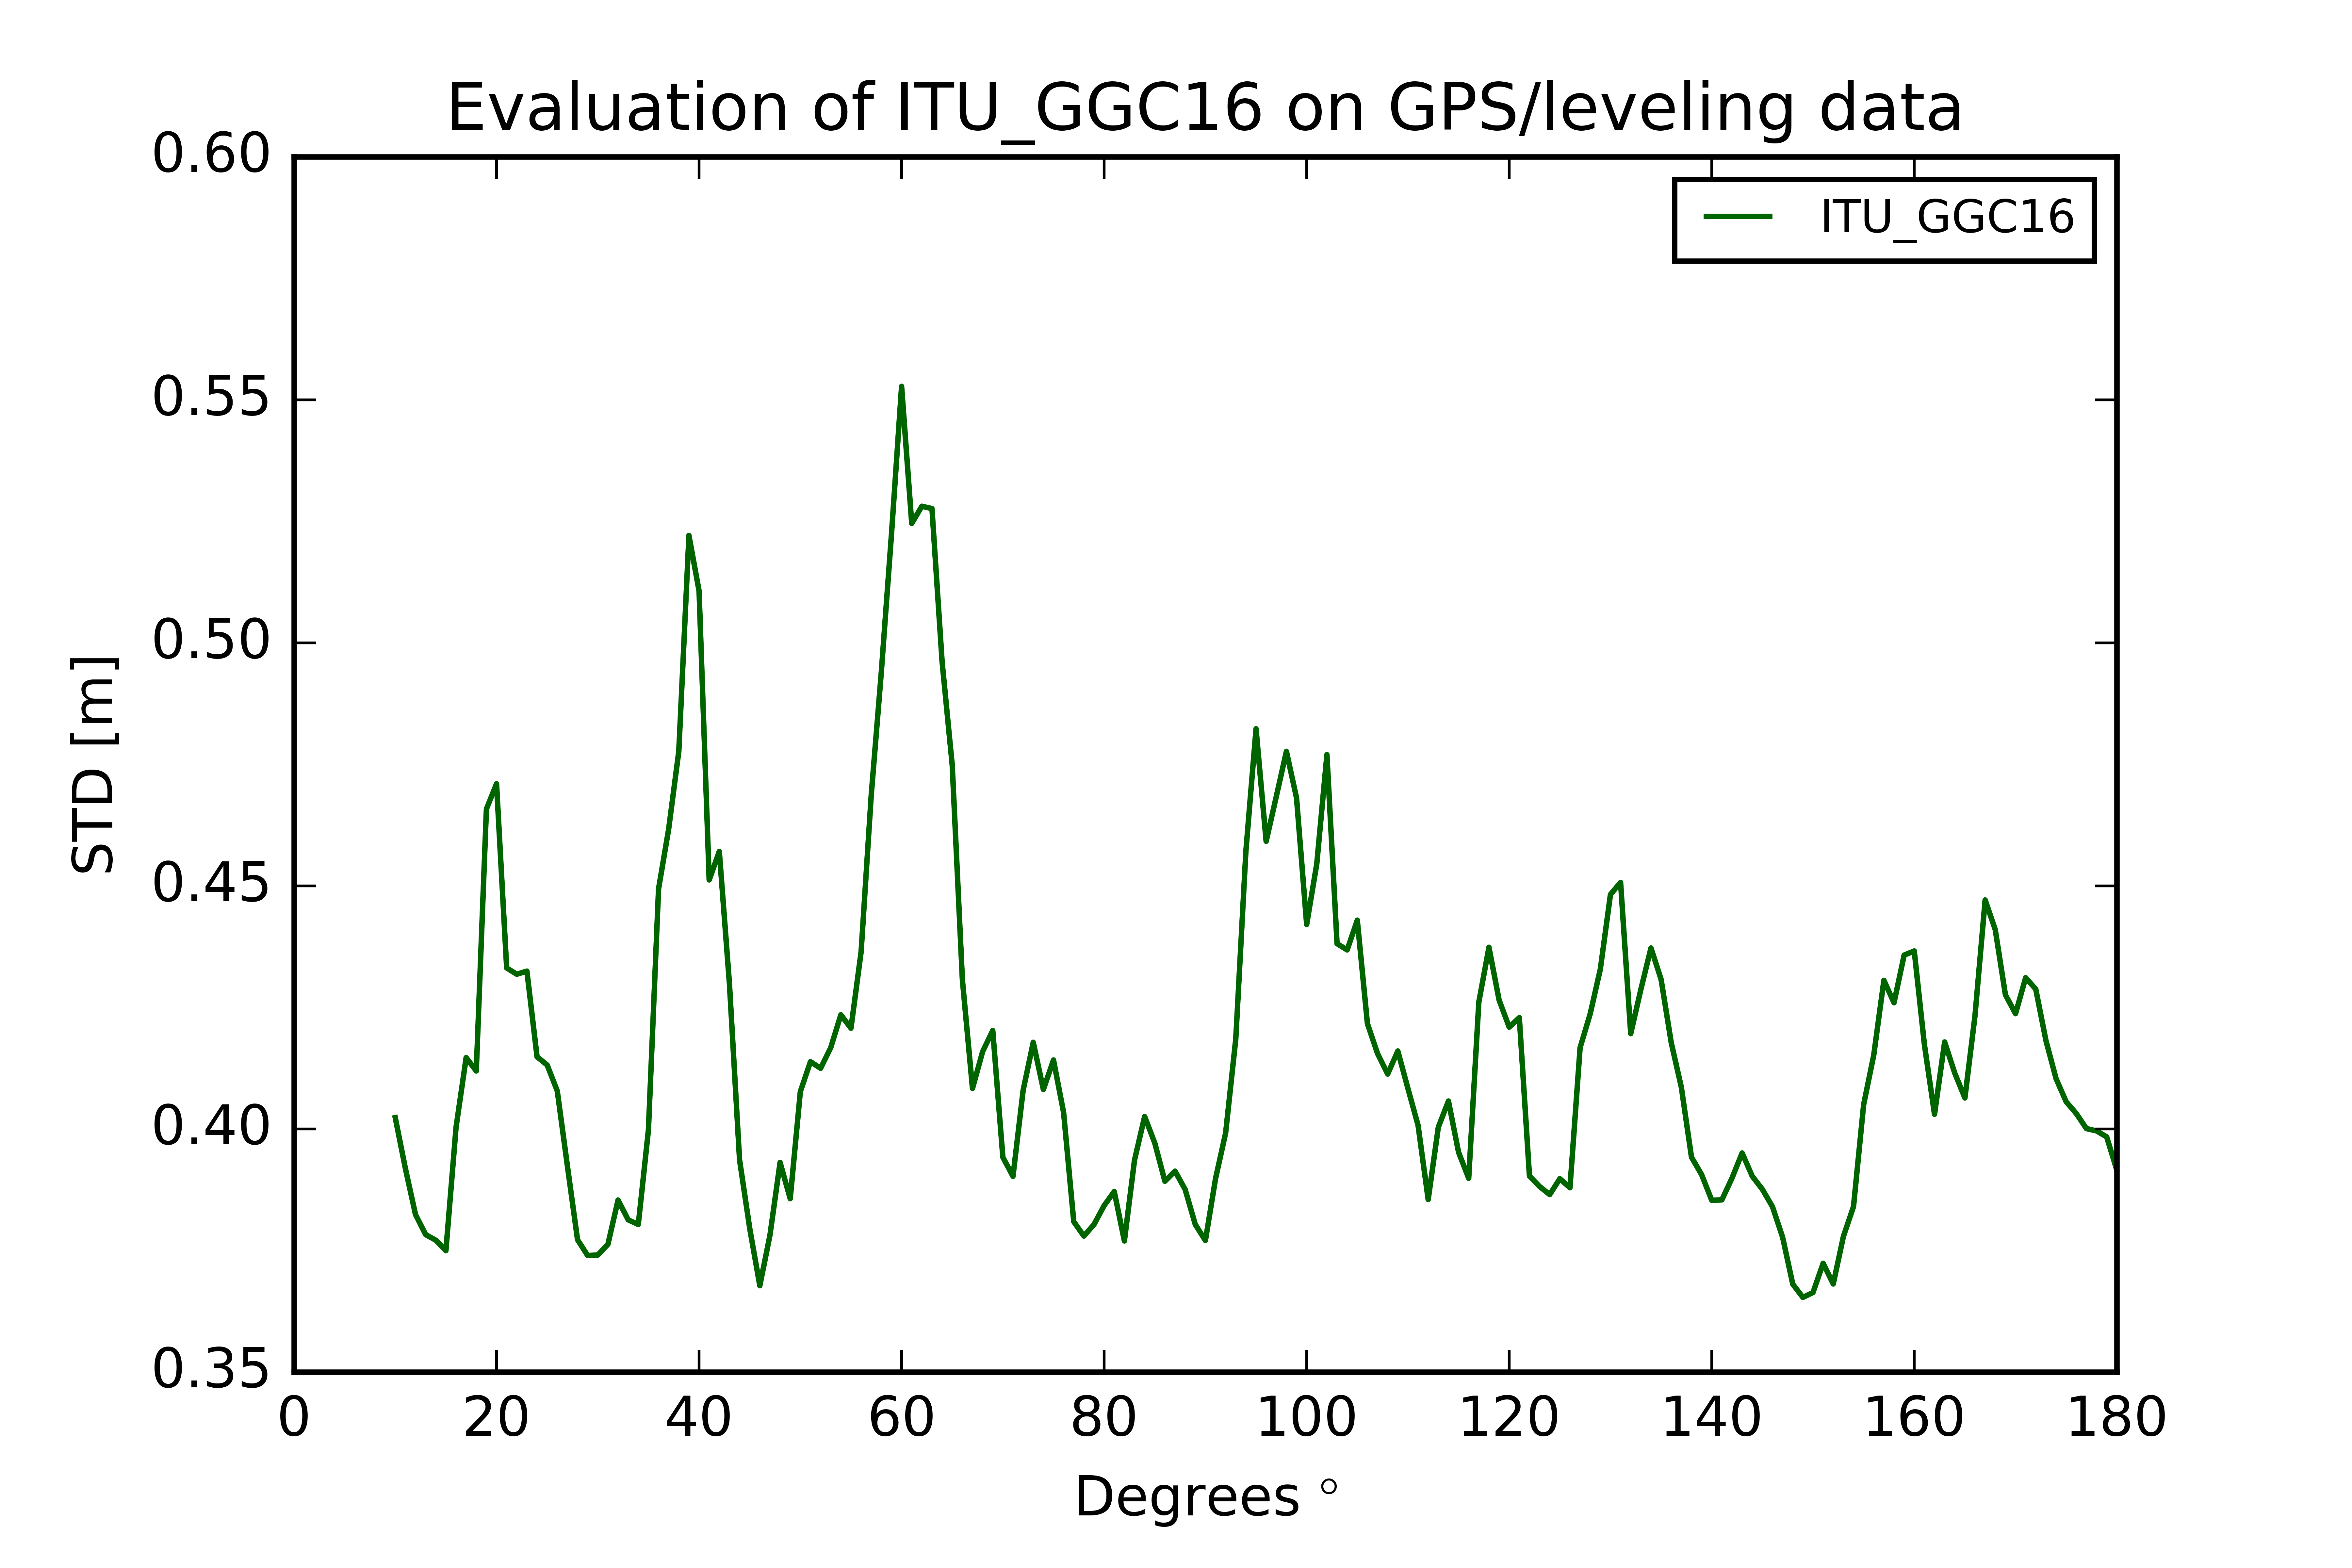
\includegraphics{Figures/ITU_GGC16_gps_figure.png}
        	\centering
        \end{figure}
        
        
        \begin{figure}[t]
        	\caption{Evaluation of GECO on GPS/leveling data}
        	\label{sudan_data}
        	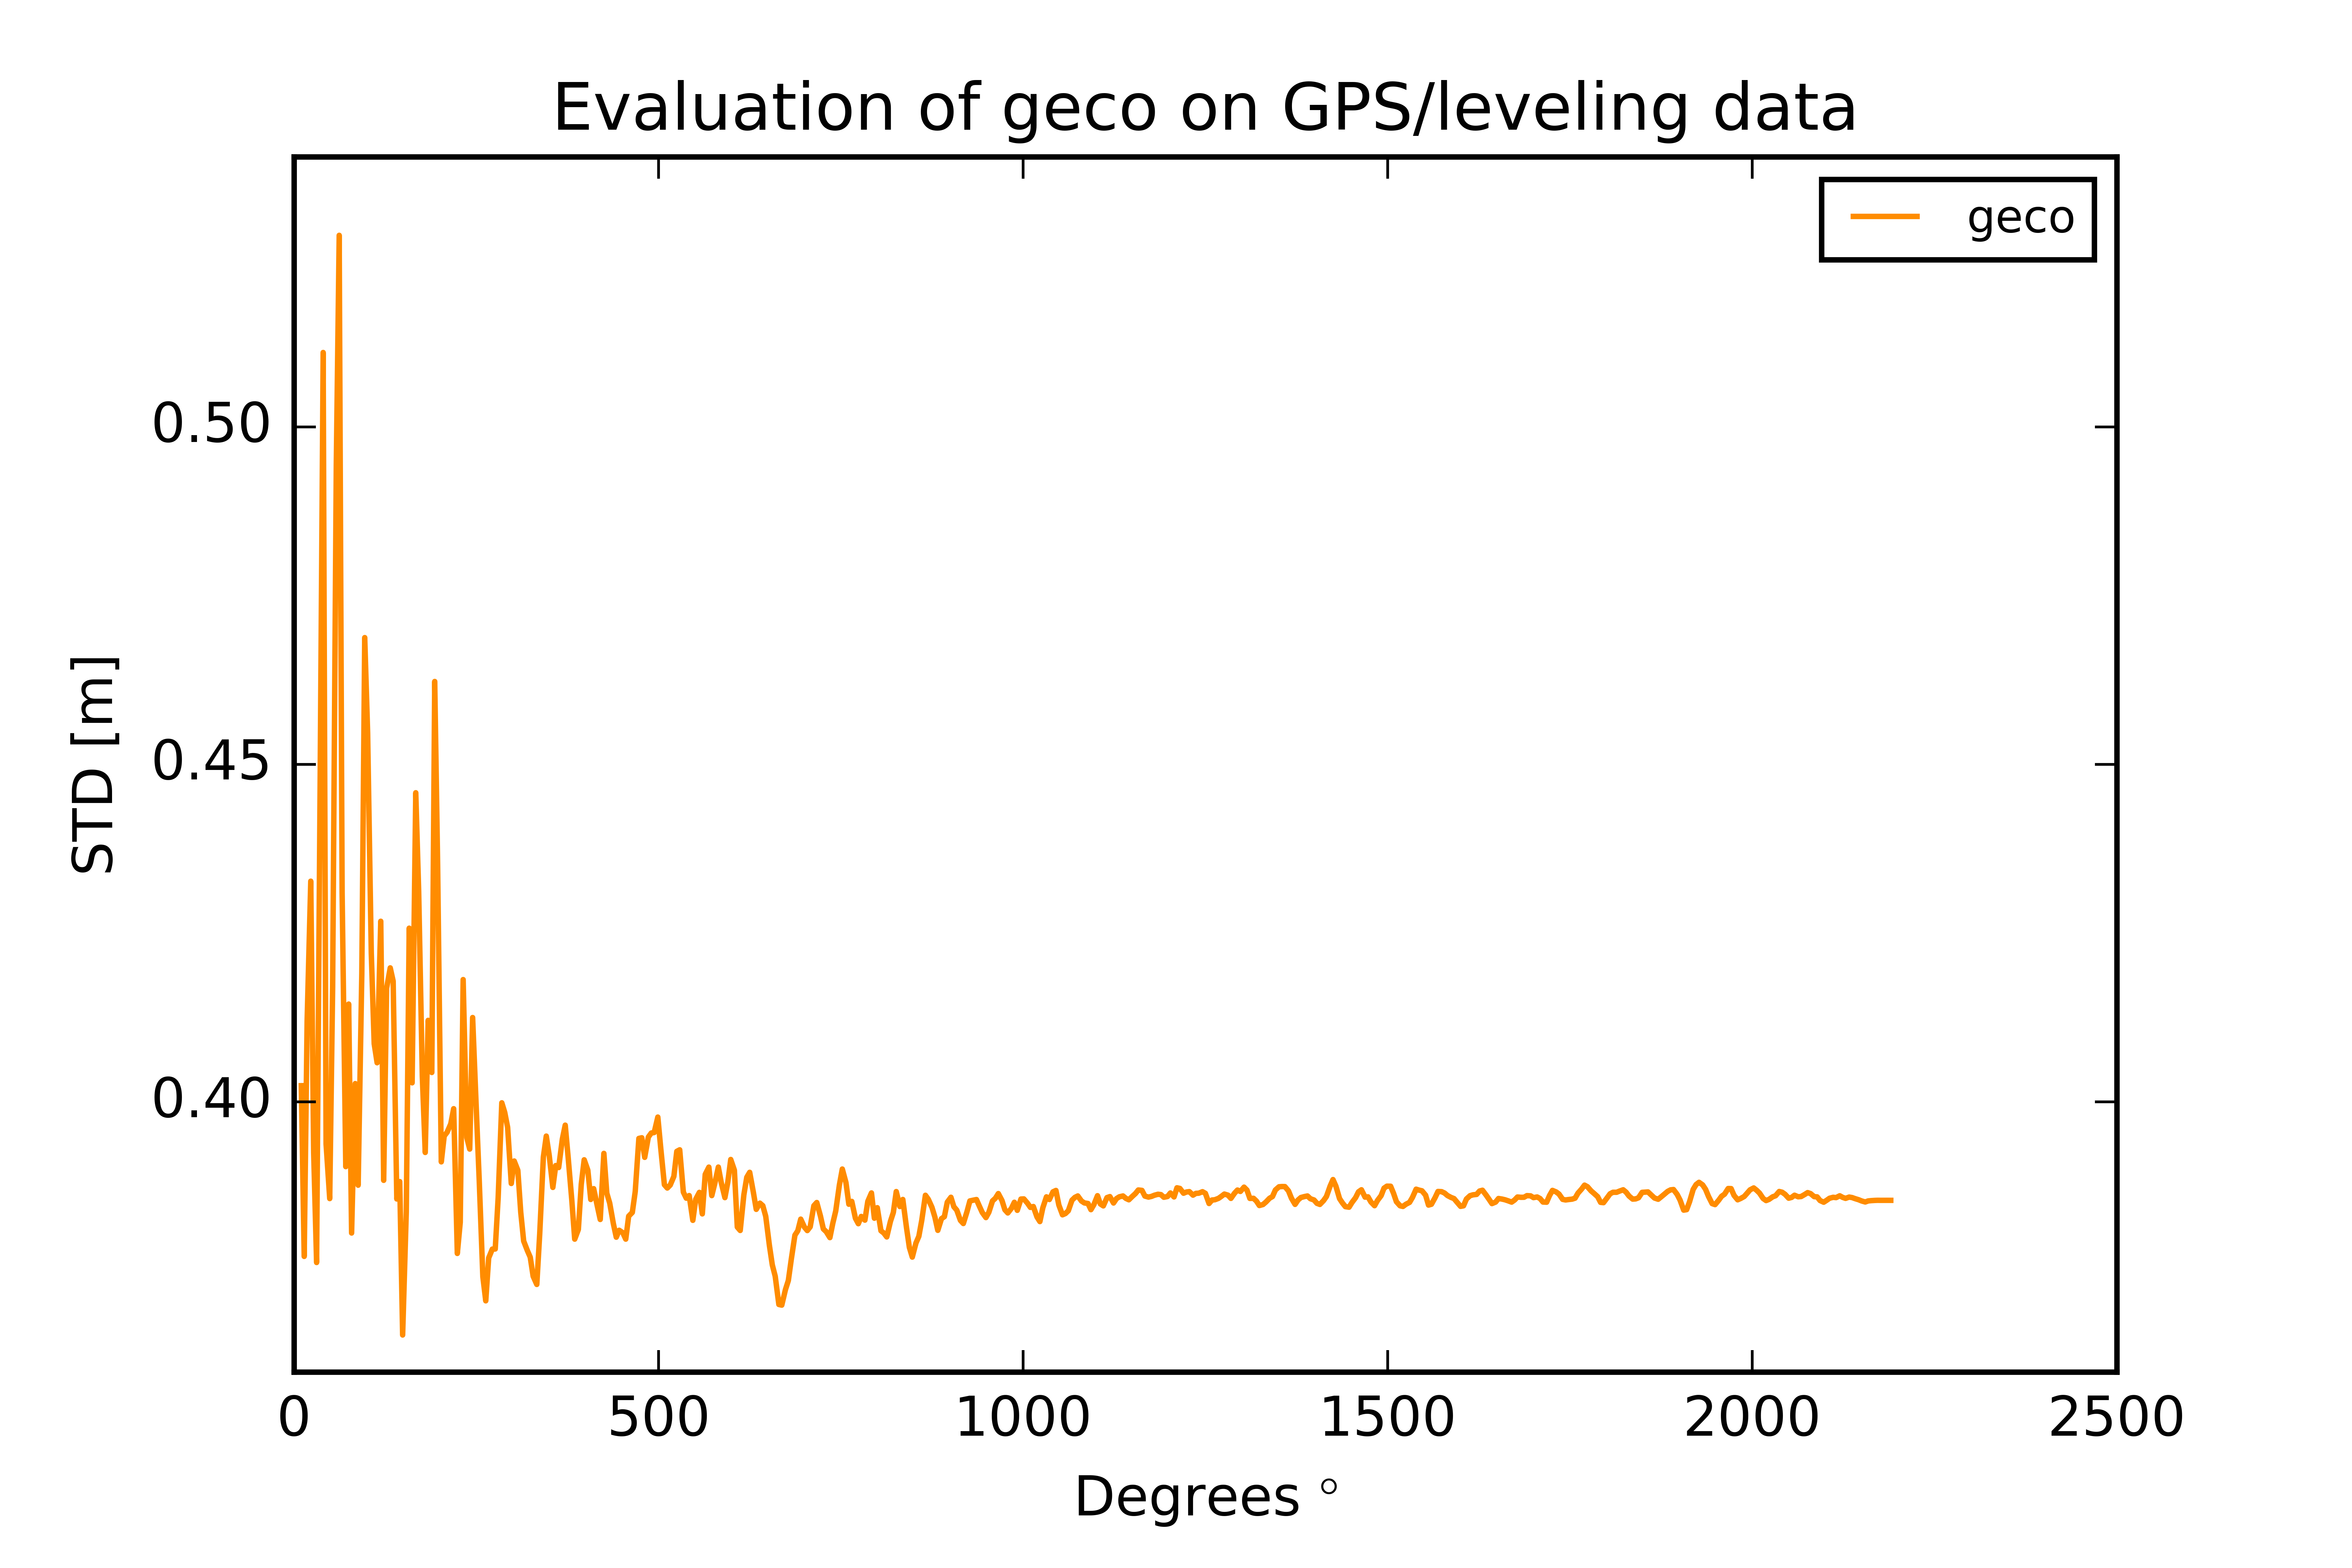
\includegraphics{Figures/geco_gps_figure.png}
        	\centering
        \end{figure}
        
        \begin{figure}[t]
        	\caption{Evaluation EIGEN-6c4 on GPS/leveling data}
        	\label{sudan_data}
        	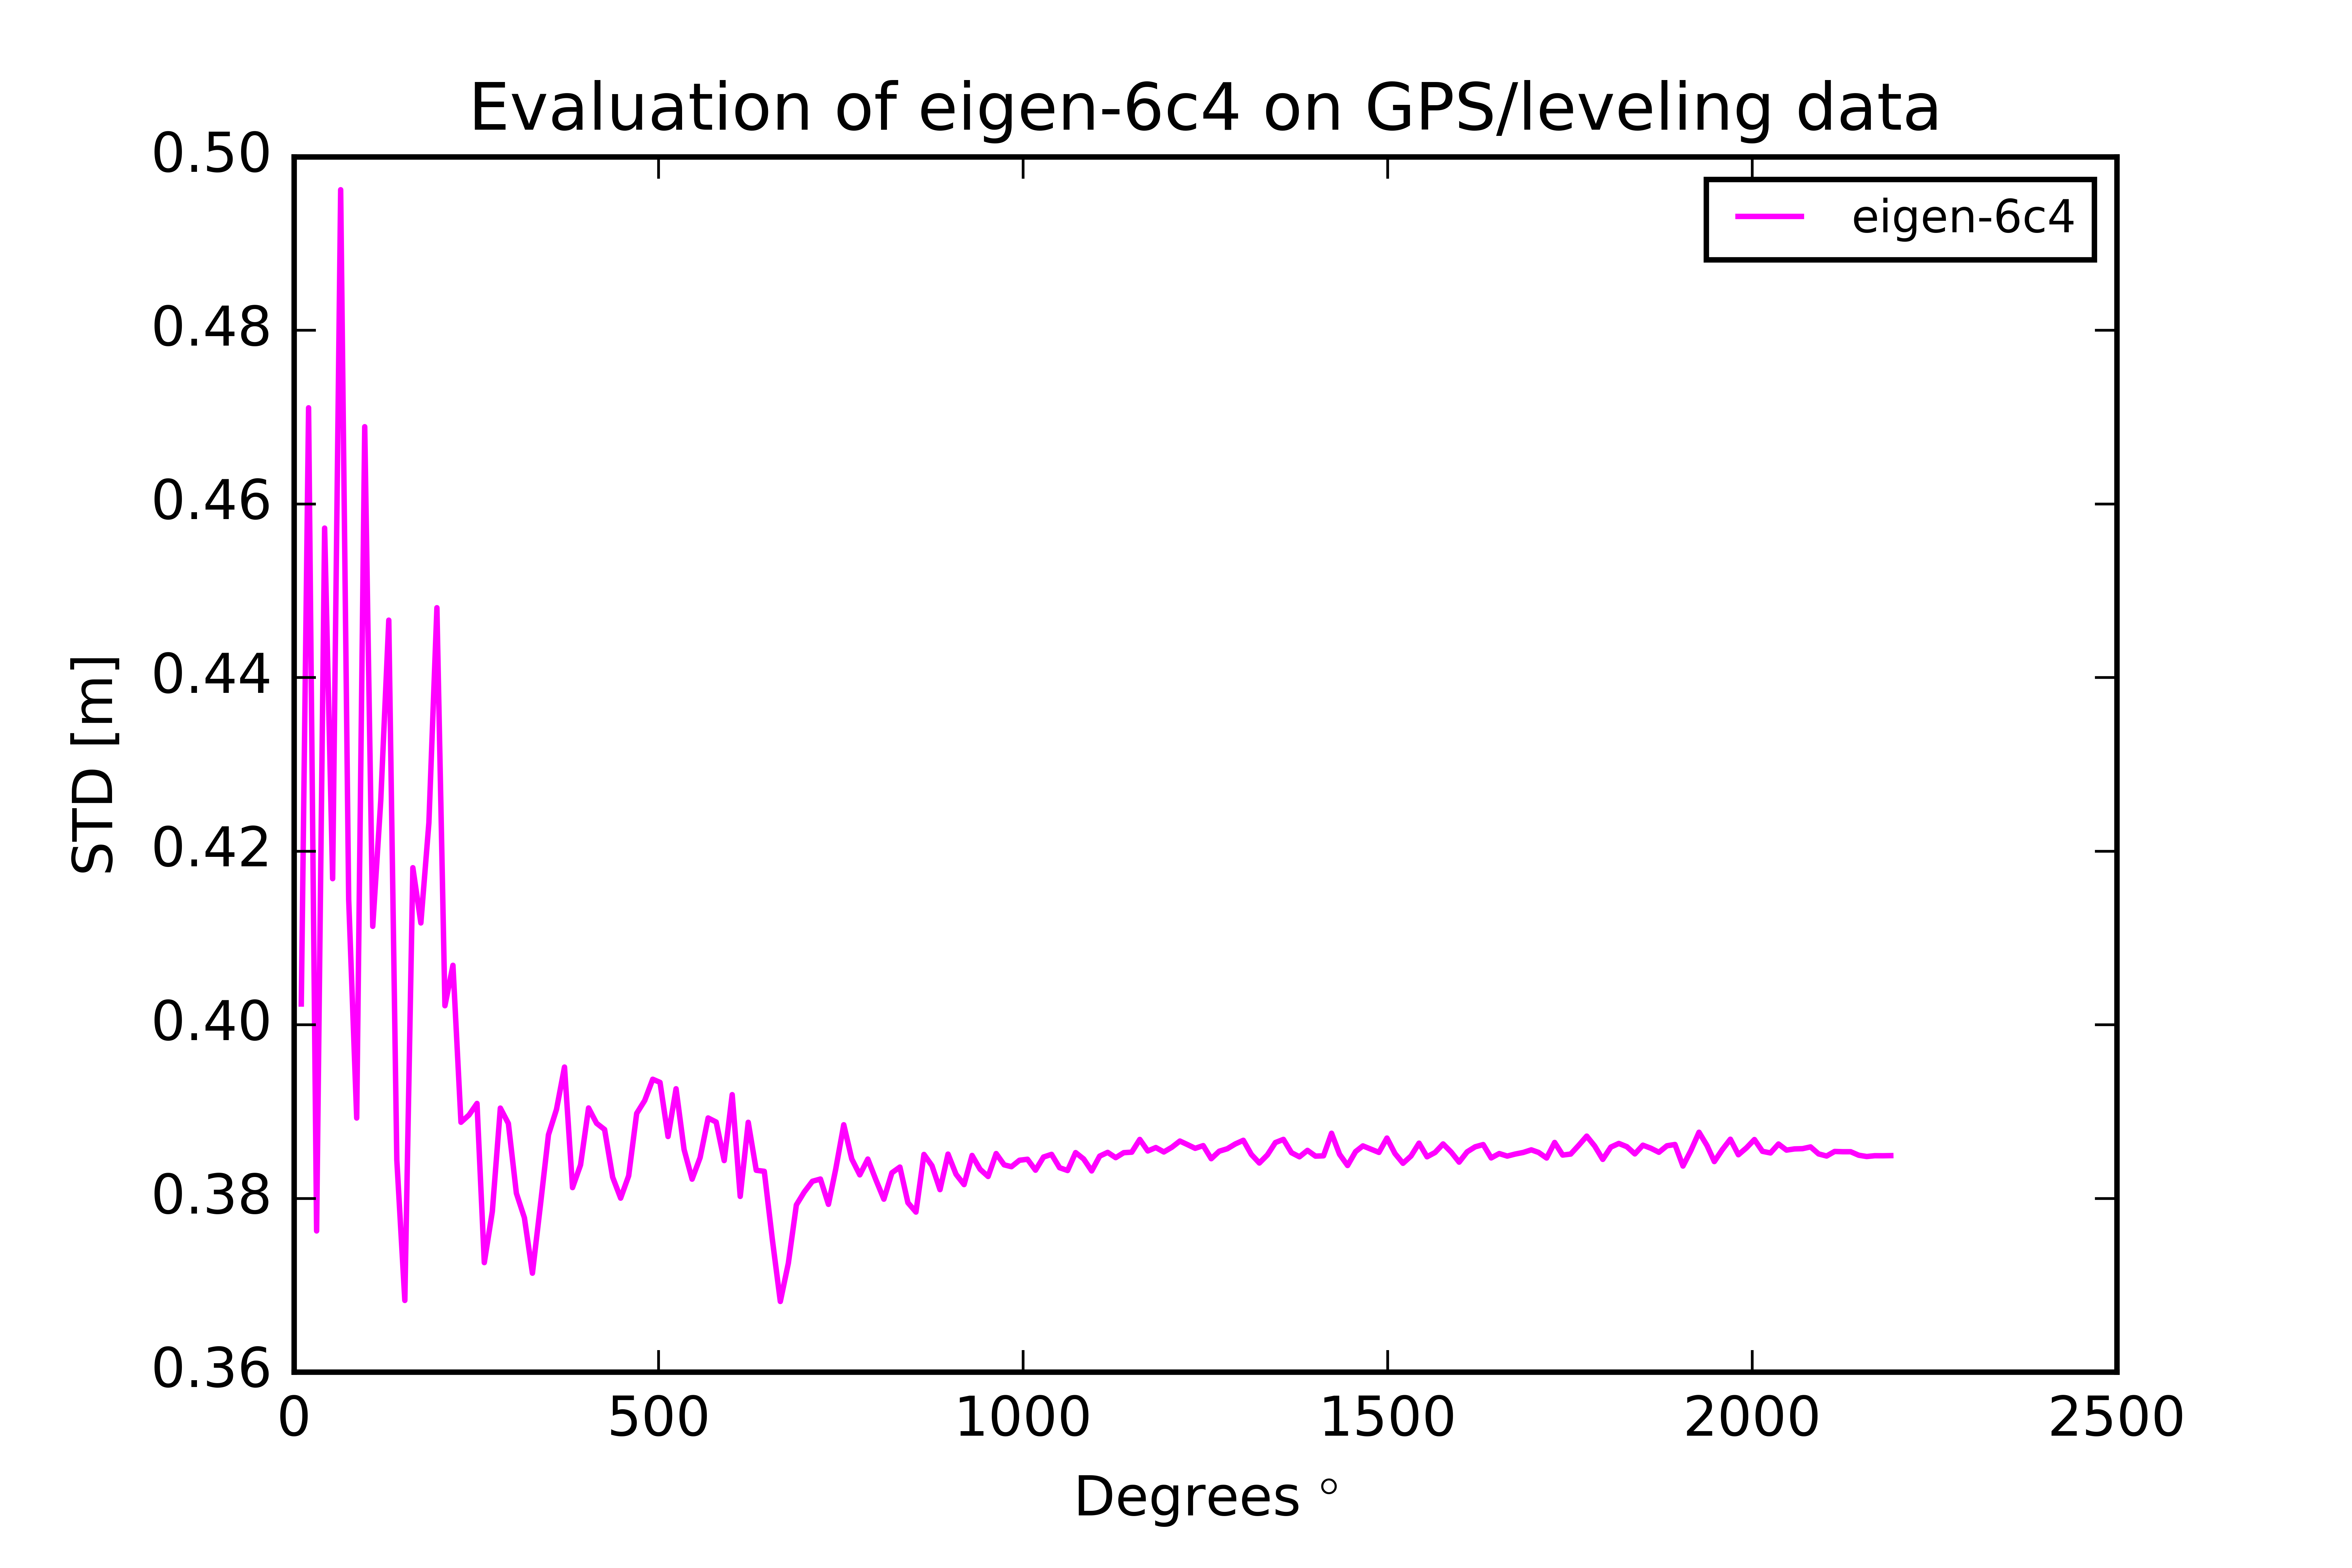
\includegraphics{Figures/eigen-6c4_gps_figure.png}
        	\centering
        \end{figure}
        
        \begin{figure}[t]
              	\caption{Evaluation of higher degrees of EGM2008, EIGEN-6C4 and GECO}
              	\label{sudan_data}
              	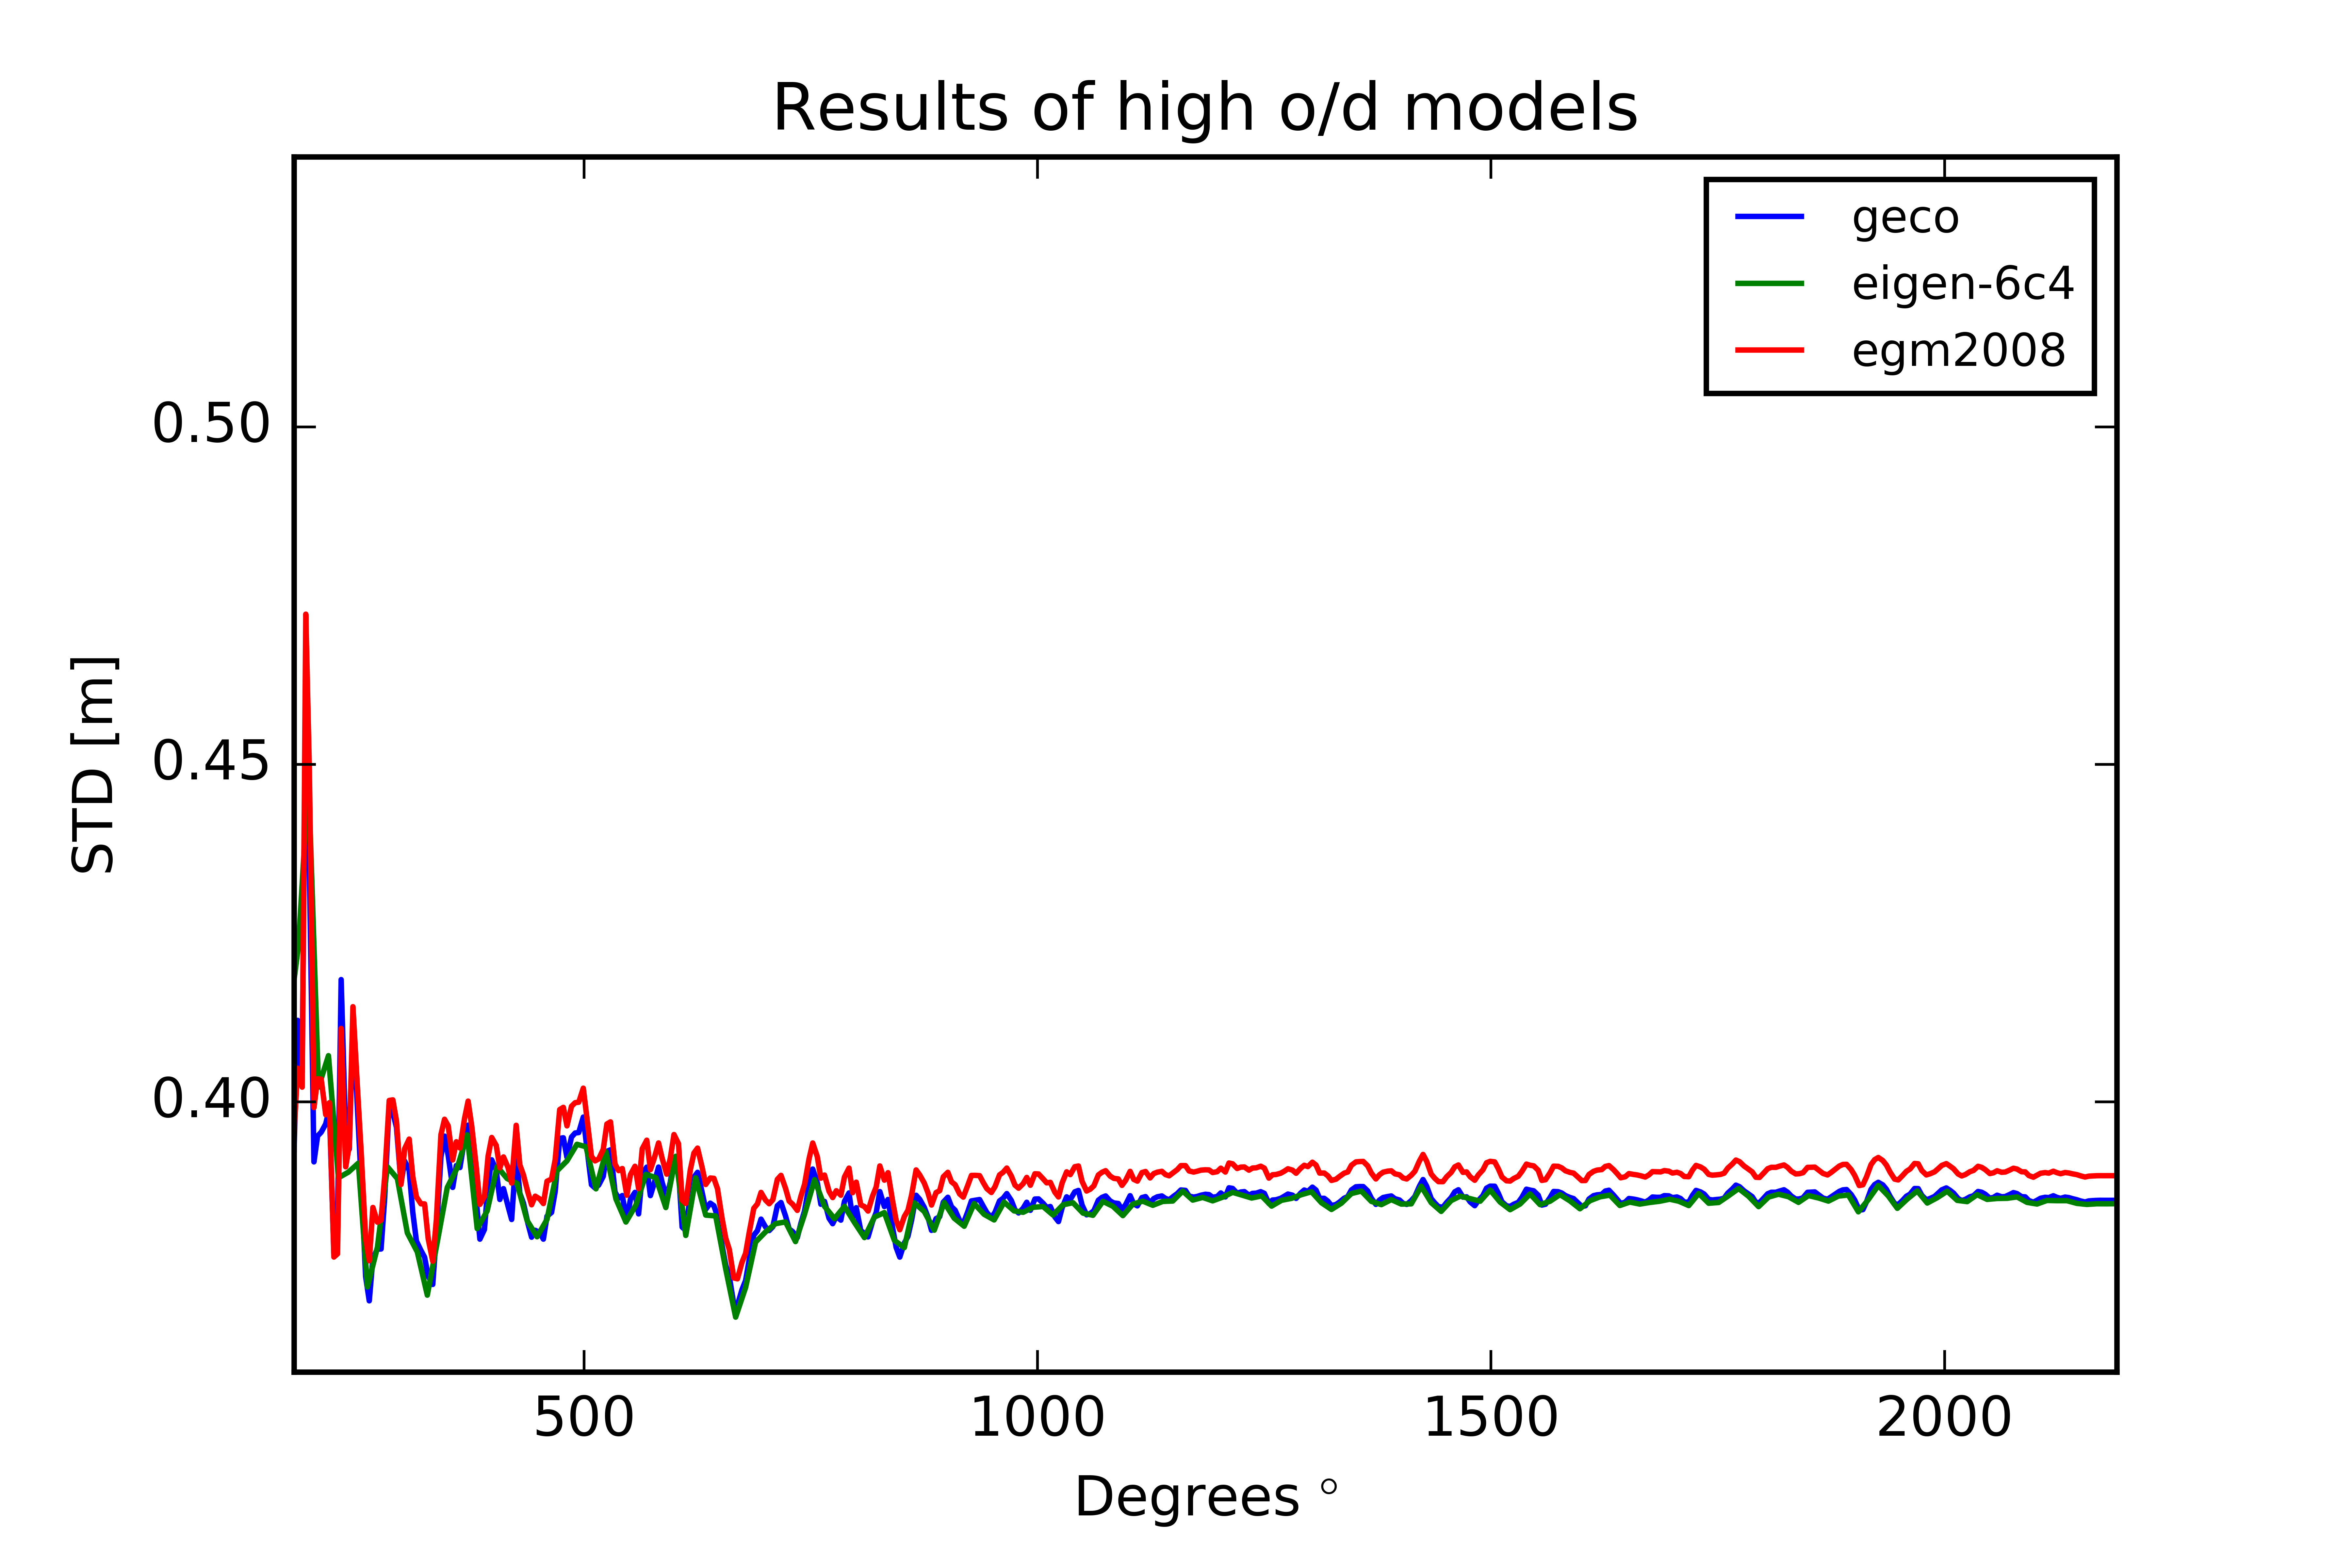
\includegraphics{Figures/high_order_results.png}
              	\centering
        \end{figure}